% Copyright (C)  2016 Philipp Hacker.
% Permission is granted to copy, distribute and/or modify this document
% under the terms of the GNU Free Documentation License, Version 1.3
% or any later version published by the Free Software Foundation;
% with no Invariant Sections, no Front-Cover Texts, and no Back-Cover Texts.
% The lincense itself can be found at <https://www.gnu.org/licenses/fdl-1.3>.

\documentclass[a4paper,10pt,twoside]{article}

\usepackage{lipsum}
\usepackage{multicol}

\usepackage[T1]{fontenc}
\usepackage[utf8]{inputenc}

\usepackage[infoshow]{tabularx}
\usepackage[all]{xy}

\usepackage{geometry}
\geometry{%
	a4paper,
	left=24mm,
	right=24mm,
	top=24mm,
	bottom=24mm,
	}

\usepackage{amsmath,mathtools}
\usepackage{amssymb}
\usepackage{units}
\usepackage{upgreek}
\usepackage{graphicx}

\usepackage{float}
\usepackage{lscape}

\usepackage[labelfont=bf]{caption}
\usepackage{wrapfig}
\usepackage{subcaption}

\usepackage[backref=page]{hyperref}

\usepackage{csquotes}
\usepackage[infoshow]{tabularx}
\usepackage{fancyhdr}

\usepackage{sectsty}
\usepackage{times}

\usepackage{lmodern} %TODO Schriftart
\usepackage[greek,english]{babel} %TODO Sprache einstellen

\renewcommand{\headrulewidth}{0.15pt}
\renewcommand{\footrulewidth}{0.15pt}
\newcommand{\name}{\text{Philipp Hacker}} %TODO Name des Protokollanten eintragen

\newcommand{\degree}{^\circ}
\newcommand{\diff}{\textnormal{d}}
\newcommand{\tenpo}[1]{ 10^{#1}}
\newcommand{\greek}[1]{\greektext#1\latintext}
\newcommand{\ix}[1]{_\text{#1}}
\newcommand{\imag}{\mathbf{i}}
\newcommand{\tilt}[1]{\textit{#1}}
\newcommand{\grad}[1]{\textit{grad}\left(#1\right)}
\newcommand{\divergenz}[1]{\textit{div}\left(#1\right)}
\newcommand{\euler}{\mathnormal{e}}
\newcommand{\fett}[1]{\textbf{#1}}
\newcommand{\ket}[1]{|#1\rangle}
\newcommand{\bra}[1]{\langle#1|}

\newcommand{\HRule}{\rule{\linewidth}{0.5mm}} % New command to make the lines in the title page

\author{Philipp Hacker} % Your name, this is used in the title page and abstract, print it elsewhere with \author

\newcommand{\prof}{Prof. Dr. Meichsner}

\newcommand{\supname}{Dr. S. Nemschokmichal, R. Tschiersch} % Your supervisor's name, this is used in the title page, print it elsewhere with \supname

\newcommand{\univname}{Ernst-Moritz-Arndt University Greifswald} % Your university's name and URL, this is used in the title page and abstract, print it elsewhere with \univname

\newcommand{\deptname}{Institute of Physics} % Your department's name and URL, this is used in the title page and abstract, print it elsewhere with \deptname

\newcommand{\groupname}{Low-temperature Plasma Physics group} % Your research group's name and URL, this is used in the title page, print it elsewhere with \groupname

\newcommand{\rtitle}{Electric field strength spectroscopy in dielectric barrier discharges}

\date{\today}


\pagestyle{fancy}
\fancyhead[R,L,C]{}
\fancyfoot[R,L,C]{}
\fancyhead[RO]{\today}
\fancyhead[RE]{\href{http://www.physik.uni-greifswald.de/}{\deptname}}
\fancyhead[LO]{\href{http://www1.physik.uni-greifswald.de/}{\groupname}}
\fancyhead[LE]{\today}
\fancyfoot[LO, RE]{\thepage}
\fancyfoot[LE, RO]{Section \thesection}

\setlength{\belowcaptionskip}{-0.4cm}
\setlength{\parindent}{0cm}

\begin{document}
	
	\renewcommand*{\contentsname}{Table of Contents}
	\renewcommand*{\equationautorefname}{eq.}
	\renewcommand*{\figureautorefname}{fig.}
	\renewcommand*{\tableautorefname}{tab.}
	\renewcommand*{\sectionautorefname}{section}
	\renewcommand*{\subsectionautorefname}{section}
	\renewcommand*{\subsubsectionautorefname}{section}
	\renewcommand*{\figurename}{Fig.}
	\renewcommand*{\tablename}{Tab.}

	\renewcommand*{\figurename}{Figure}
	\renewcommand*{\tablename}{Table}

	
	\thispagestyle{empty}
	
	\begin{center}
			
			\HRule \\[0.4cm] % Horizontal line
			\huge \fett{\rtitle} \\[0.3cm] %TODO TITLE
			\large  -- Report for an internship -- \\ %TODO UNIVERSITY TEXT
			\HRule \\[.4cm] % Horizontal line

			\small submitted by \\
			\large \href{https://github.com/RayleighsJeans/ag_praktikum_2016}{\name}\\[0.2cm] %TODO TITLE AUTHOR NAME

			\begin{figure}[h]
				\centering
				
				\begin{minipage}[t]{0.48\textwidth}
					\flushleft
						\href{http://www1.physik.uni-greifswald.de/}{\groupname} \\ %TODO GROUPNAME
						\href{http://www.physik.uni-greifswald.de}{\deptname} \\ %TODO DEPARTMENT
						\href{http://www.uni-greifswald.de}{\univname} \\ %TODO UNIVERSITY
						Felix-Hausdorf-Str. 6, 17489 Greifswald
				\end{minipage}
				\hfill
				\begin{minipage}[t]{0.48\textwidth}
					\flushleft
						\emph{Supervisors}: Dr. S. Nemschokmichal and \\ \hspace{1.9cm} R. Tschiersch \\ %TODO name of supervisor
						\hspace{0.175cm} \emph{Examiner:} \prof
				\end{minipage}
			\end{figure}

	\end{center}
	
	\begin{multicols}{2}
		\tableofcontents
	\end{multicols}
	
		\vspace{0.75cm}
	
		\paragraph{Abstract}
		
	\twocolumn

	\section{Introduction}\label{sec:intro}

		In the vast field of low-temperature plasma physics, barrier discharges (BDs) play a key role for applications at elevated pressures, as a result of their unique feature of surface charge deposition onto, the dielectric-covered electrodes. During the discharge breakdown, the accumulated charges limit the overall current, as they attenuate the opposing electric field across the gas gap. Furthermore, by that means the resulting plasmas are thermally non-equilibrated, even at atmospheric pressures. Barrier discharges act as a source of radicals, excited species and high energy electrons and photons. Actually, a variety of working gases and their mixtures can be used to force a variety of different discharge modes, each yielding characteristic physical quantities, obtainable through, e.g. non-invasive optical spectroscopy or electrical measurements.\\ 
		Barrier discharges are very lucrative for the industry due to their comparatively low power consumption, low electron temperatures and easy-to-achieve viability. Especially high quality productions, for example surface treatments, gas synthesis, or in life science benefit from those properties. Besides the technical importance, certain properties of dielectric hindered, atmospheric-pressure, low-temperature plasmas, like short, non-stationary breakdown times and therefore fast repeatability, statistical behavior and non-thermal distribution functions, motivate the intense study of the various phenomena found in BDs.\\
		By variation of the discharge configurations, such as electrode spacing, applied voltage, gas flow and mixture and dielectric material, BDs can be operated as filamentary micro discharges (\tilt{MD}s), which appear as thin, lateral constricted filaments, or in diffuse modes. The latter are subject of the present investigation. Here, one can distinguish between the atmospheric pressure Townsend-like discharge (\tilt{APTD}) and the atmospheric pressure glow-like discharge (\tilt{APGD}).\\
		\tilt{APGD}s are mostly investigated in rare gases with high ionization inside the discharge volume at a low electric field strength. Essentially, elementary multistage processes of such noble gases account for many metastable species, which are found to be crucial for charge carrier generation by Penning ionization. A unique feature is the development of a cathode fall region during the breakdown.

			\begin{figure}[t]
				\centering
				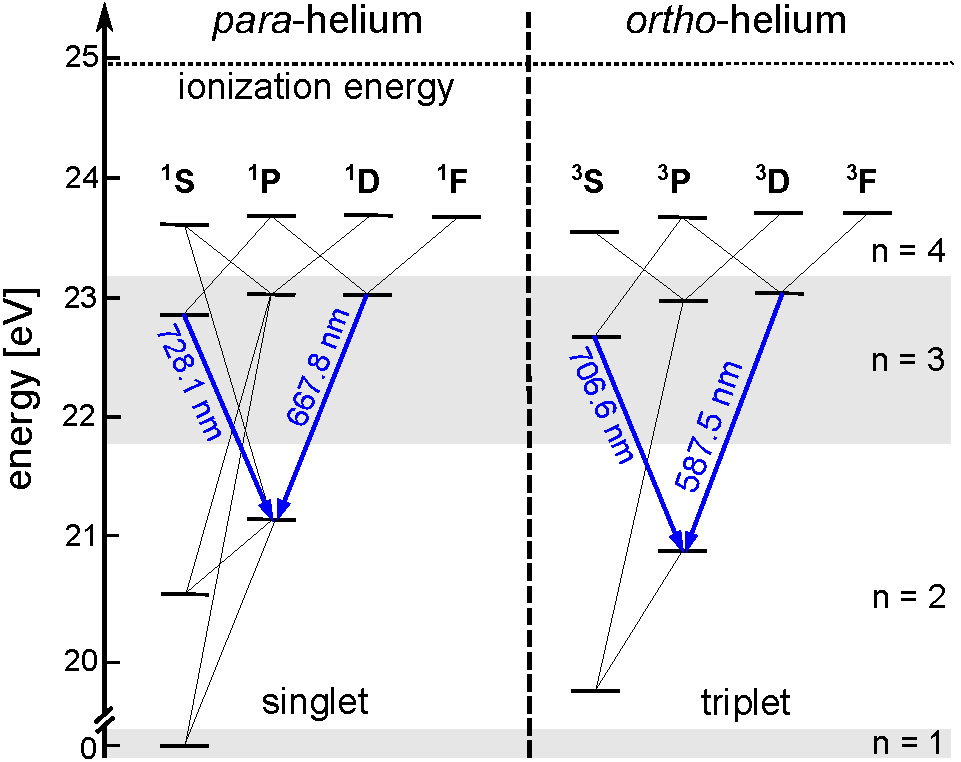
\includegraphics[width=0.5\textwidth]{figures/setup/He_energy_diagram.pdf}
				\caption{Energy diagram of helium for singlet and triplet transitions. Our used lines are emphasized. Here, we only refer to the second and third shell of para- and ortho-helium.}
				\label{img:termnschema}
			\end{figure}
		
		\tilt{APTD}s are result of a high ratio of secondary electron emission to volume ionization. This is caused by the Townsend breakdown at the cathode, primarily in gases with metastable species which have enough energy to produce secondary electrons, yielding an exponential growth of electron density towards the anode.\\
		The Townsend-like and the glow-like discharge separate each other by a difference in transferred current during the breakdown of at least one order of magnitude. In addition to the measurement of external quantities, electron temperatures, plasma currents and densities or produced species, the spatially resolved investigation of the resulting electric field strength, and therefore related characteristics like optical emission and life time become cruel to the true understanding of the discharge. Concretely, any macroscopic electric fields in plasmas are result of space charge formation. Their characteristics commonly determine the energy flux of charged particles and therefore, the behavior of the discharge itself. \\
		On the one hand, electric field strength measurements through experimentally determined emission intensity ratios of SPS/FNS have been appointed as standard, though this method is limited to a small range of nitrogen to oxygen ratios. On the other hand, for a long time, experimental fusion devices rely on the helium line intensity ratio method to determine the electron density, temperature and the local electric field strength. In fact, electron impact excitations are insensitive to electron density but to electron temperature. If one uses the ratio of two line intensities excited in the plasma, the electron density factor gets cancelled out and what remains is only dependent on the electric field strength. Hence, this method can also be used to obtain a field strength distribution in spatially small dielectric barrier discharges at low temperatures and atmospheric pressures.\\
		In this case, Helium is used, as the singlet spin state weakly depends on an initial metastable population, since He(singlet) is effectively transferred into He(triplet). A collisional-radiative model has to be utilized to attain the field distribution in the cathode region of such low-temperature non-equilibrium APGD. Specifically, the used emission lines set up on He I $\unit[728,31]{nm}$ ($3^1$S-$2^1$P) and He I $\unit[667.98]{nm}$ ($3^1$D-$2^1$P) for the singlet states. In addition, we have chosen the 2 triplet states at He I $\unit[587,65]{nm}$ ($3^3$D-$2^3$P) and He I $\unit[706,66]{nm}$ ($3^3$S-$2^3$P). One should note here, that those states are not yet described by such collisional-radiative model and metastable ions can not be neglected for low electric fields states.\\
		Furthermore, a second method for electric field \linebreak strength measurement will be introduced. Stark splitting and shifting of atomic levels, therefore spectroscopic emission lines, is a well established method in plasma diagnostics. It is based solely, so to speak \tilt{ab initio} on nature, on the quantum mechanical perturbation of atomic energy levels by strong external electric fields. Hence, neither equilibrium or additional conditions have to be fulfilled, nor is the line splitting a function of further plasma properties other than field strength. Polarization filters are used to distinguish between the different $\pi$ and $\sigma$ bands, as a full spectrum may include overlaps, which can lead to misinterpretation.\\
		Here, the linear Stark effect can be applied on the splitting of $\pi$-polarized, forbidden and allowed energy levels in Helium atoms. A polynomial will be used to fit the splitting to the field strength. The allowed-forbidden gap will be investigated at around $\unit[492,2]{nm}$ for the transition 1s2p$^1$P$^0$ - 4d$^1$D$^0$ and its forbidden counterparts 2p$^1$P$^0$ - 4p$^1$P$^0$ and 2p$^1$P$^0$ - 4f$^1$F$^0$.\\
		In this report, a comparison of spatially and temporally high resolved measurements, in both the two ways mentioned above, is presented. The aim is to find a qualitative agreement in the results, as this would satisfy each methods theories, as well as the diagnostics setup. A further purpose of the outlined setup is to characterize the different discharge modes with regard to their electric field strength development during the breakdown.\\
		The outline of this report is as followed. In the next section, the experimental setup that was used and the diagnostics will be briefly reviewed. Section 3 will present and discuss selected results, associated discussion of such.

	\section{Experimental setup}
	
		\subsection{Discharge configuration}
		
				\begin{figure}
					\centering
					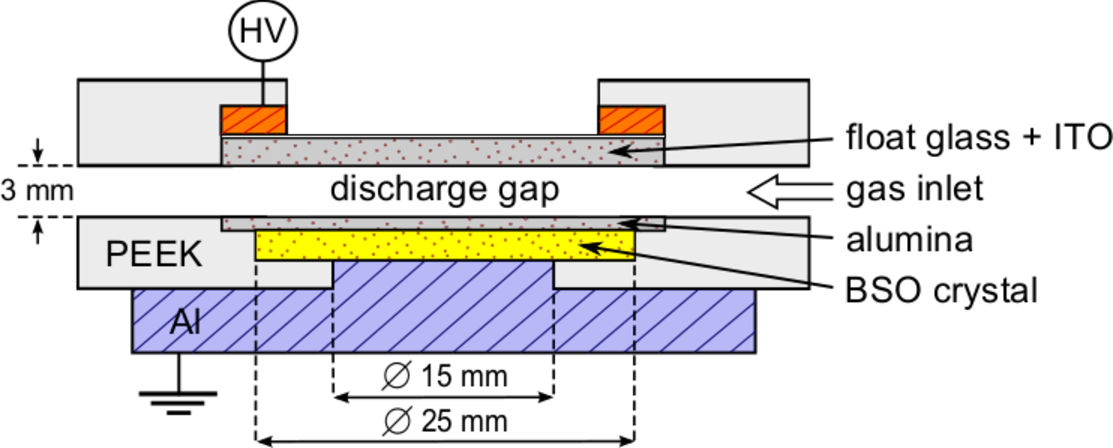
\includegraphics[width=0.5\textwidth]{figures/setup/discharge_cell.pdf}
					\caption{side-view of the concentric discharge cell. The variable dielectric was chosen to be mono-crystalline alumina.}
					\label{img:cell}
				\end{figure}
		
			The used discharge configuration is sketched in \autoref{img:cell}. Here, a symmetrical configuration, in which both plane, concentric electrodes are covered with dielectrics is used. The gas gap width is $\unit[3]{mm}$ in height, whereas the diameter of the electrode is $\unit[15]{mm}$. A high-voltage driven copper ring is on top of a float glas plate, which is thus covered with an electrically conductive, transparent indium tin oxide  (\tilt{ITO}) layer. On the bottom, a grounded aluminium mirror holds a bismuth silicon oxide (\tilt{BSO}) crystal. On top of that, a variable dielectric can be mounted, which is fixed to be aluminium in this experiment. Here, mono-crystalline alumina (Al$_2$O$_3$) was used. In advance for calculation of electrical quantities, it is crucial to know the different permittivities and dimensions of the dielectrics used in the discharge cell  - see \autoref{tab:permits}. The corresponding capacitance is calculated by $C\ix{x}=\varepsilon\ix{x}\varepsilon_0 A/2d$.\\
			The whole construct is mounted inside a steel vacuum chamber. A turbomolecular pump evacuates the chamber to a base pressure of about $\unit[\tenpo{-5}]{mbar}$, which ensures low concentration of impurities. Afterwards, the operating gas is passed from one side directly into the chamber through the polyetherethereton (PEEK) gap spacers. Two mass flow controllers (MKS 647c) set the gas flow rate of Helium and Nitrogen (respective purity > 99,999\%) achieving high-accuracy mixtures and flow rates of up to $\unit[100]{sccm}$. The discharge operated at atmospheric pressure that of $\unit[1000]{mbar}$, which was kept constant through a diaphragm pressure gauge and butterfly valve (MKS) by the process pump (TRIVAC D25BCSPFPE).
			

				\begin{table}[h]
					\centering
					\begin{tabular}{c|c|c}
						material & d/mm & $\varepsilon\ix{r}$ \\
						\hline \hline glas+ITO & 0,7 & 7,6 \\
						\hline Al$\ix{2}$O$\ix{3}$ & 0,2 & 10,55 \\
						\hline BSO & 0,7 & 56 \\
					\end{tabular}
					\caption{Physical quantities of dielectrics inside discharge cell.}
					\label{tab:permits}
				\end{table}

		\subsection{Electrical diagnostics}\label{subsec:electric}
		
				\begin{figure}
					\centering
					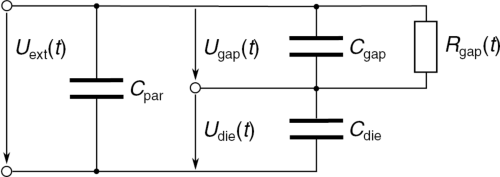
\includegraphics[width=0.5\textwidth]{figures/setup/replacementcircuit.pdf}
					\caption{Electrical equivalent circuit: the discharge gap is represented by the time-dependent resistance $R\ix{gap}(t)$ and $C\ix{gap}$ in parallel.}
					\label{img:circuit}
				\end{figure}
				
			 As shown in \autoref{img:diag}, a function generator (SRS DS345) provides the voltage signal for the upper electrode, which ignites the discharge after amplification of the voltage signal by a factor of 1000 (Trek 615-10), at a frequency of $\unit[5]{kHz}$ and amplitude of $\unit[1,2]{kV}$. The voltage can be a sine or square wave, which has influence on the discharge modes.\\
			 Applied voltage $U\ix{app}(t)$ and total transported charge $Q\ix{ext}$ are measured via a HV probe of (1000:1) and an external capacitor, $C\ix{ext}=\unit[1]{nF}$. The monitoring and averaging of data is performed by a digital oscilloscope (ROHDE\&SCHWARZ RTO1024) with a bandwidth of $\unit[2]{GHz}$, which is connected through ethernet ports to a PC, running a customized LabView VI. Additionally, a Rogowski coil is attached to the cell, accumulating the flowing current and providing a much faster and higher slope. This signal also is used as the trigger for the oscilloscope.\\
			 Furthermore, by using Lissajous figures $Q(U)$, one gains access to the transported charge $\Delta Q$ during the breakdown and the determination of the total capacitance of the discharge cell $C\ix{tot}$. By that, the gap voltage between the dielectrics $U\ix{gap}$ and the discharge current $I\ix{dis}$ can be calculated \cite{Kogelschatz2003}. A electrical equivalent circuit can be constructed, as depicted in \autoref{img:circuit}. Here, $C\ix{die}$ and $C\ix{gap}$ denote the capacitance of the dielectrics and discharge gap, taking into account the geometry. The parallel capacitance $C\ix{par}=C\ix{tot}-C\ix{gap}C\ix{die}/\left(C\ix{gap}-C\ix{die}\right)$ comprehends any volume in the cell not ignited by the discharge. Additionally, the barrier discharge capacitance $C\ix{BD}$ is defined as the parallel and dielectric capacitance in series. One can calculate the described quantities and yields \autoref{tab:capac}.
			 
				\begin{align}
					 U\ix{gap}(t)=&\left(1+\frac{C\ix{par}}{C\ix{die}}\right)U\ix{app}(t)-\frac{Q\ix{ext}(t)}{C\ix{die}} \,\, , \\
					 I\ix{dis}(t)=&\left(1+\frac{C\ix{gap}}{C\ix{die}}\right)\times \nonumber \\
					 &\left(\frac{\diff Q\ix{ext}(t)}{\diff t}-C\ix{tot}\frac{\diff U\ix{app}(t)}{\diff t}\right) \,\, .
				\end{align}	

				\begin{table}
					\centering
					\begin{tabular}{c|c}
						quantity & C/pF \\ \hline\hline
						$C\ix{Al2O3}$ &  82,54 \\ \hline
						$C\ix{glas+ITO}$ & 16,99 \\ \hline
						$C\ix{BSO}$ & 125,17 \\ \hline
						$C\ix{gap}$ & 0,52 \\ \hline
						$C\ix{par}$ & 2,01 \\ \hline
						$C\ix{die}$ & 12,66 \\ \hline
						$C\ix{BD}$ & 0,51 \\ \hline
						$C\ix{tot}$ & 2,51 \\
					\end{tabular}
					\caption{Capacities of the presented discharge configuration.}\label{tab:capac}
				\end{table}
	
		\subsection{Optical emission spectroscopy}\label{subsec:oes}
		
				\begin{figure}
					\centering
					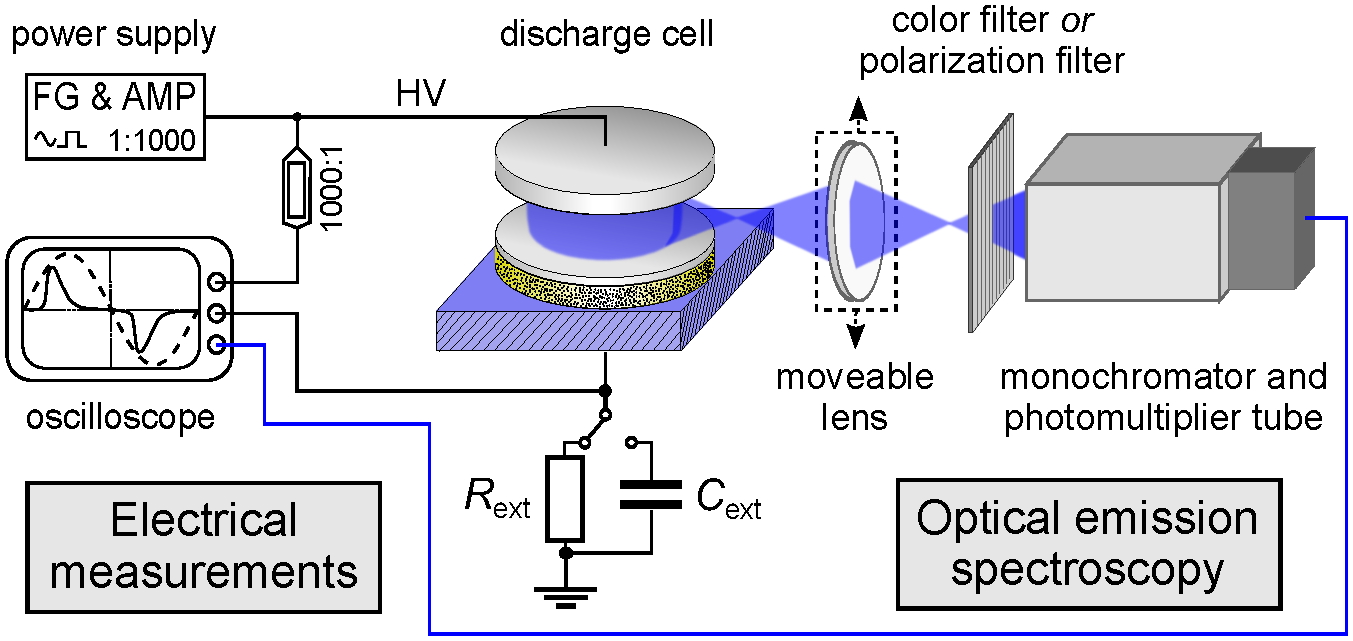
\includegraphics[width=0.5\textwidth]{figures/setup/setup.pdf}
					\caption{Set-up of the diagnostics used, with the corresponding discharge cell configuration.}
					\label{img:diag}
				\end{figure}
		
			The \autoref{img:diag} illustrates the diagnostic setup, by which the simultaneous investigation of electrical quantities, like charge and current, as well as the optical emission from the discharge is possible.\\		Here, the spatio-temporally resolved acquisition of single photons is accessible through a high-gain photomultiplier (PM: HAMATMATSU photomultiplier tube R928; length $\unit[0,75]{m}$), a 1:1250 amplifier and monochromator. The fully movable optical system of two lenses, one slit and three vernier screws for vertical and horizontal adjustments across the full discharge cell, is focused via 1:-1 onto the monochromator (MC: Horiba, HR320) with an entrance slit of $\unit[3]{mm}$. In this case, a step width of $\unit[0,1]{inch}$ or $\unit[0,15]{inch}$ is chosen. Through the combination of rogowski coil and digital oscilloscope a temporal resolution down to $\unit[2]{ns}$ is achieved. With a grating of $\unit[2400]{mm^{-1}}$, the monochromator achieves a spectral resolution of $\unit[0,02]{nm}$ at comparatively low intensities. At $\unit[1800]{mm^{-1}}$ one yields a lower resolution with higher photomultiplier currents.\\
			As the discharge frequency was chosen to be $\unit[5]{kHz}$, many data acquisitions per second can be performed by the digital oscilloscope. As the PM achieves a individually distinguishable electric signal for each photon, the raw data from the PM and amplifier has to be averaged over thousands of inner loops - for example 28000 averages at a sample rate of $\unit[100]{MSa/s}$ to cancel out any background noise. In addition, outer loops will be performed to rule out medium-range perturbations.\\
			For the line emission intensity ratio spectroscopy, the monochromator first scans a full spectrum between $\unit[585]{nm}$ and $\unit[730]{nm}$, including all Helium lines of interest. Specifically, those will be the already mentioned lines from triplet states at $\unit[587,65]{nm}$, $\unit[706,66]{nm}$, as well as singlet states with $\unit[728,31]{nm}$, $\unit[667,98]{nm}$. Surprisingly, those lines come with a small offset of $\approx\unit[0,15]{nm}$, compared to values obtained from various literature - see for example \href{http://www.nist.gov/pml/data/asd.cfm}{NIST Atomic Spectra Database} \cite{NIST_ASD}. This will be further discussed in the next section.\\
			While the line ratio measurement is performed at a single wavelength, the Stark spectroscopy needs the recording of a small window of $\unit[0,7]{nm}$ in $\unit[0,02]{nm}$ steps. Therefore, the spectral resolution is much higher, whereas the spatial resolution was reduced to $\unit[0,2]{inch}$ to get satisfying intensities.\\
			Both methods use the same setup, but differ in application. During the line emission spectroscopy, the optical system is elevated each time the measurement of all four lines is completed. Therefore, the entrance and exit slit of the MC are widened to $\unit[0,2]{mm}$, while the slit height remains $\unit[0,1]{mm}$. The cell gap is scanned with $\unit[0,05]{inch}$ steps.\\
			For Stark spectroscopy, the entrance/exit slit width and height are at $\unit[0,1]{mm}$, $\unit[3]{mm}$,with a lower vertical resolution of $\unit[0,1]{inch}$. The grating was $\unit[2400]{mm^-1}$ here. Furthermore, the already mentioned polarization filter is placed along the optical axis between the MC and discharge cell.

	\section{Results}

		\subsection{Overview spectrum of optical emission}\label{subsec:overview}
			
				\begin{figure}
					\centering
					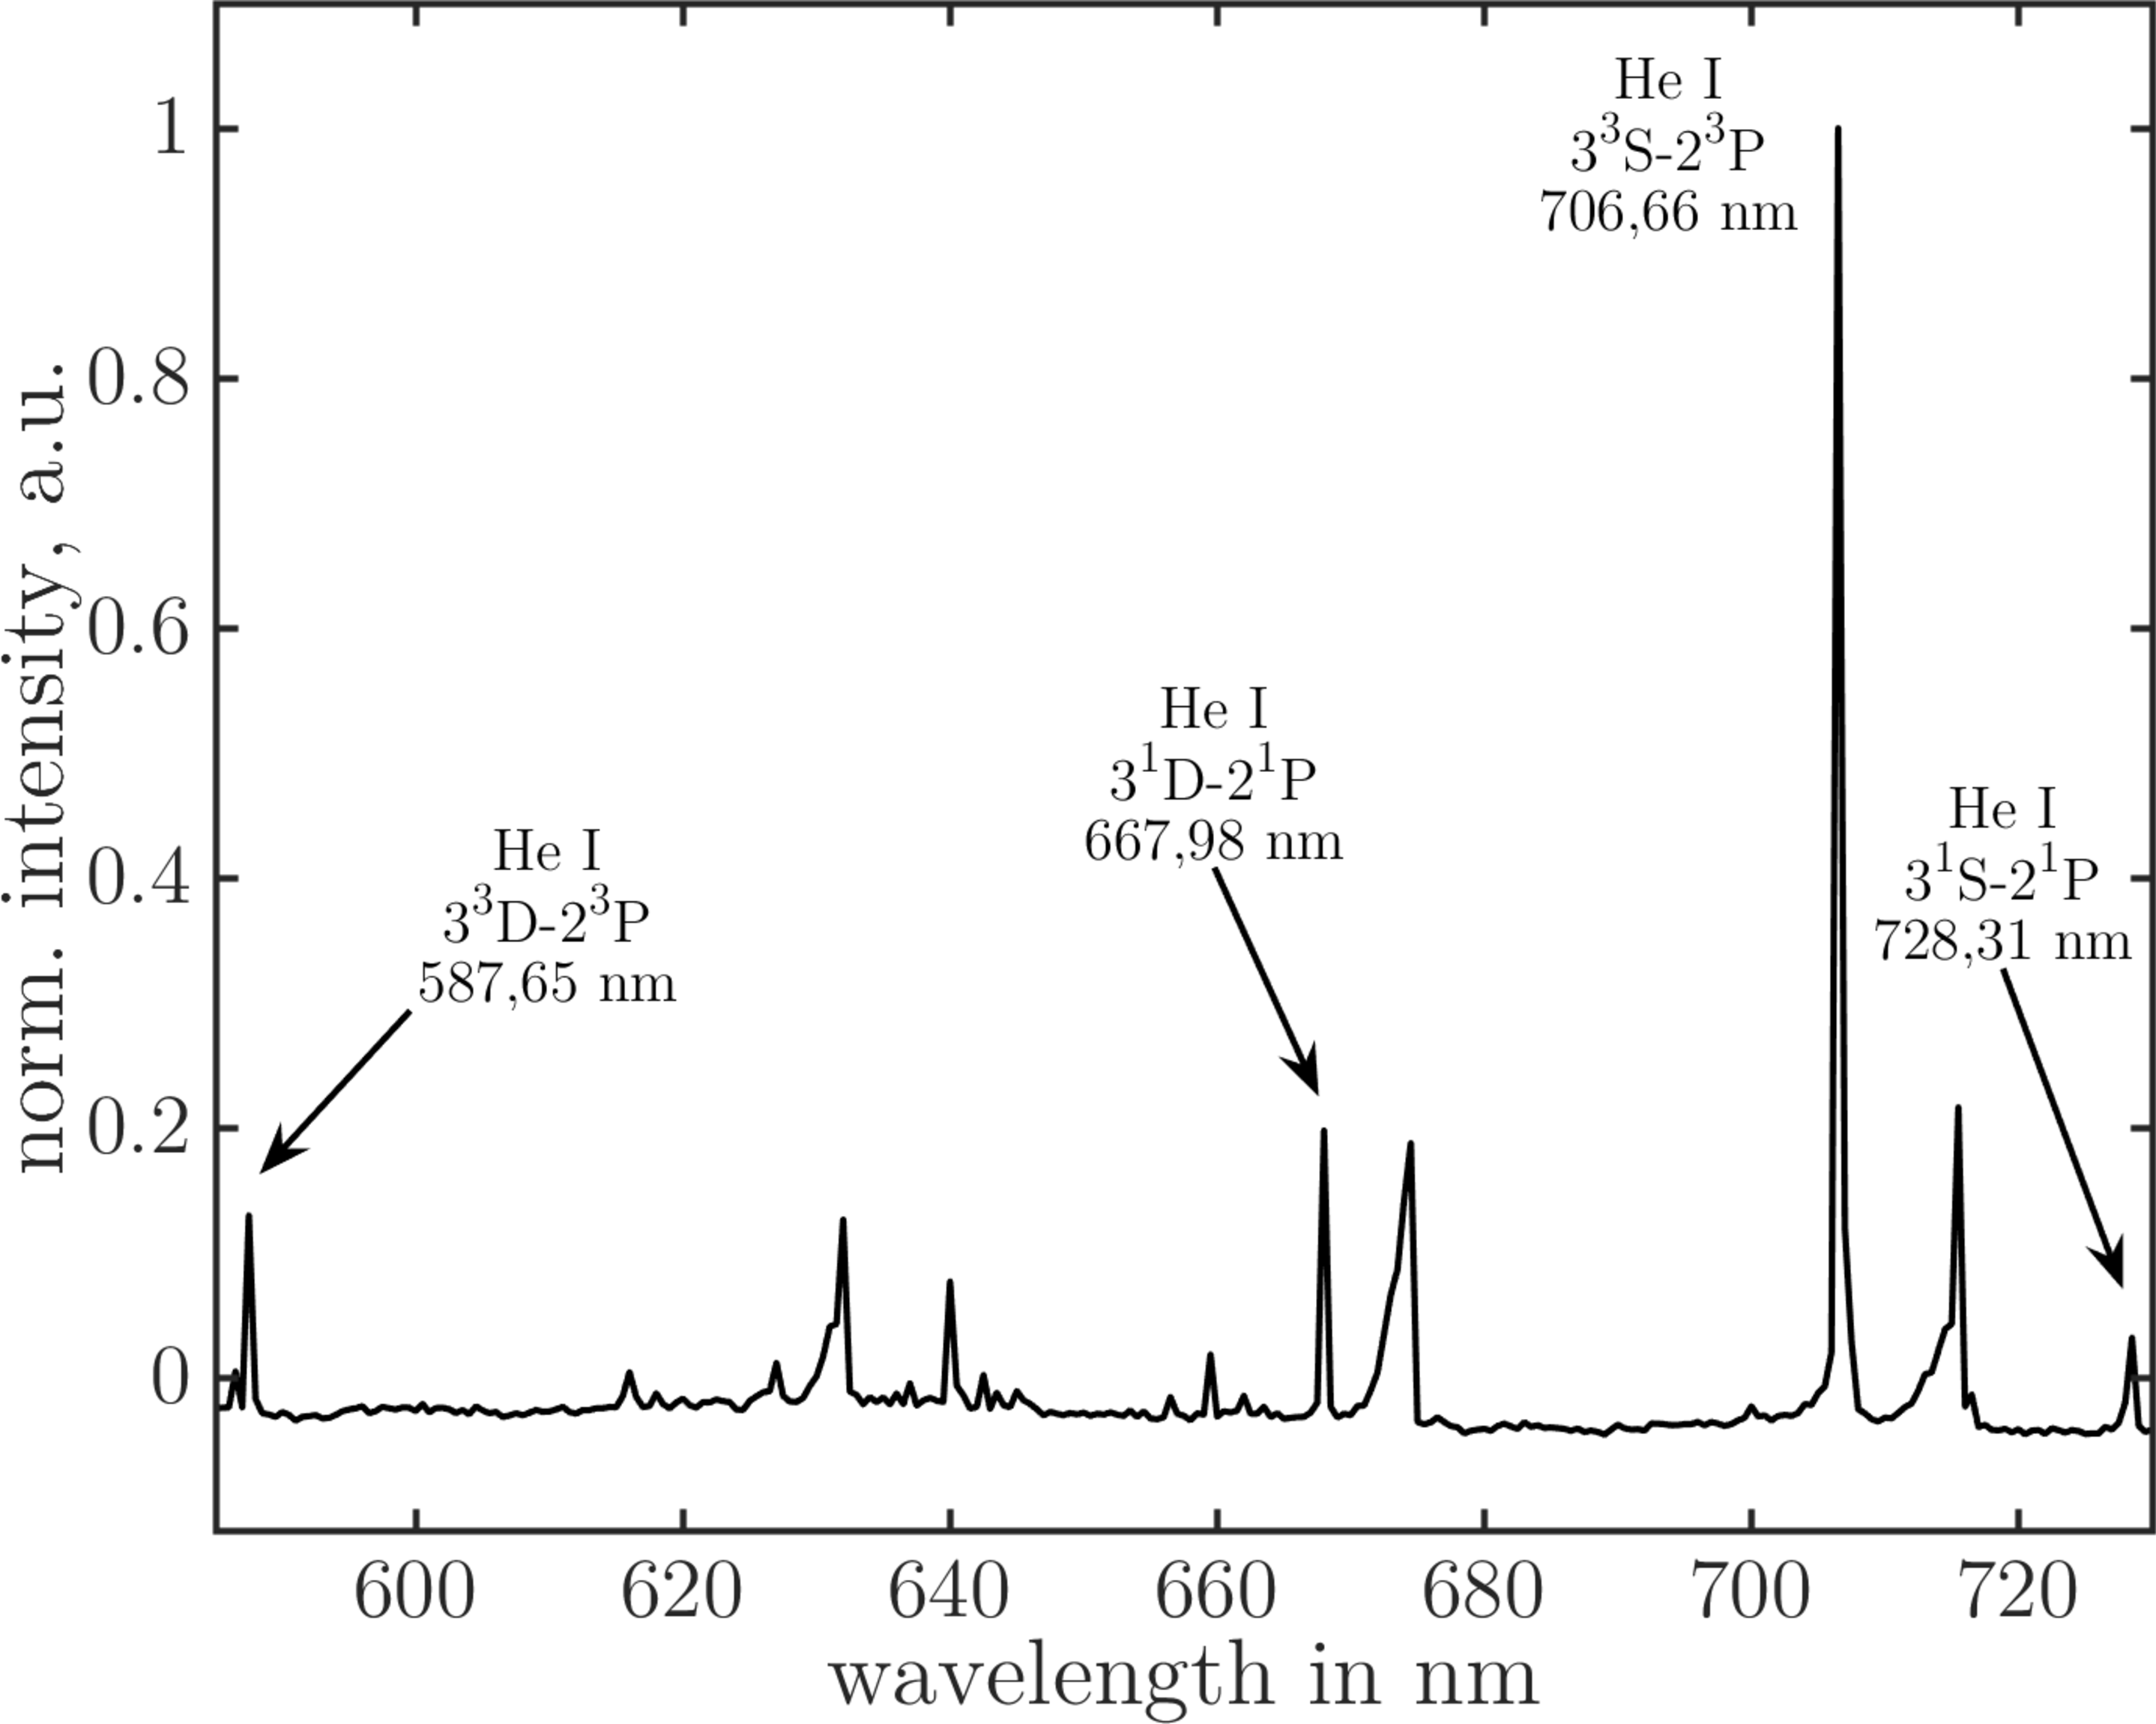
\includegraphics[width=0.5\textwidth]{figures/results/int_spectrum}
					\caption{Overview spectrum for a BD of $\unit[100]{sccm}$ He$_2$ and $\unit[0,05]{sccm}$ N$_2$ at a pressure of $\unit[1]{bar}$. Applied Voltage $\unit[1,2]{kV}$ at $\unit[5]{kHz}$.}
					\label{img:intspec}
				\end{figure}
		
			During this experiment, a mixture of $\unit[100]{sccm}$ helium and $\unit[0,05]{sccm}$ nitrogen, with a purity of $>99,999\%$ was used. The discharge has been excited and ignited by a square wave of $\unit[5]{kHz}$ with an amplitude of $\unit[1,2]{kV}$, and kept at a constant, atmospheric pressure of $\unit[1]{bar}$ by the mass flow controller. Additionally, the optical set-up was configured for high intensities at comparatively decent resolution. Therefore, a grating of $\unit[1800]{mm^{-1}}$ with $\unit[0,5]{nm}$ spectral resolution and a slit opening of $\unit[3]{mm}, \unit[0,2]{mm}$ width and height.\\ 
			An overview spectrum is presented in \autoref{img:intspec}. Here, the transitions discussed before in \autoref{sec:intro} are highlighted. Those will be indeed the subject of the spatio-temporally resolved line emission spectroscopy in \autoref{subsec:stroe}.\\
			The full spectrum, ranging from $\unit[585]{nm}$ to $\unit[730]{nm}$ was then corrected by its offset and integrated. The dark range between $\unit[592]{nm}$ and $\unit[612]{nm}$ was used to calculate the offset. Afterwards, a simple numerical integration method was applied to the spectrum (see \cite{Wiki:Euler}). Thus, the temporal dimension is resolved, yielding the spectrum from \autoref{img:intspec}.\\
			This figure contains the positions and quantum mechanical transition terms for peaks, which have already been singled out in \autoref{sec:intro}. Primarily, these lines are found to be the dominant ones in our spectrum. Especially, the transition from $3^3$S to $2^3$P carries the maximum intensity measured. The spectrum includes emission lines from relaxation of excited singlet or triplet states of helium.\\
			As shown in, e.g. \cite{linratio1_14}, the excitation of mentioned states is induced by impacting electrons, which are generated in regions of high electric field strength. Therefore, these electrons have a higher kinetic energy and hence, correspond directly to the field strength and intensity of the given transitions. Furthermore, the intensity ratios between the $\unit[667,98]{nm}$ line and $\unit[728,31]{nm}$ are also independent of local densities. This is due to the equal influence of the electron numbers to all excitation states.\\
			During low field strength phases of the discharge, excitation from metastable levels becomes more important. This is due to the low electron impact energy, which is then too low for the direct electron impact excitation of the $n=3$ levels.. Therefore, in any later evaluations one has to keep in mind, that the used model lacks a proper interpretation for low electric field strengths and the corresponding intensity in emission.\\
			To get a more detailed look at the physical background, one has to look at the de-/ population of the named states. On the one hand, intensities of singlet lines mostly originate from the ground level $2^1$P, whereas the effect of metastables is negligible here. On the other hand, triplet line emission is strongly affected by metastable densities, especially in regions of low electric field strength. Furthermore, electron impact excitation of the ground and metastable levels, $2^1$S and $2^3$S, populate the above states. Excitation from the triplet $2^3$S to singlet levels is highly unlikely. Vice versa, the excitation from $2^1$S is orders of magnitude more probable, contributing to the intensity of such triplet states. Therefore, the intensities of states populated from the ground level $2^3$S are much more significant than those of the spin counterpart $2^1$S, see \autoref{img:termnschema}. Additionally, transitions between 3P and 3D have been taken into account in following models.\\
			Depopulation is happening through spontaneous emission and associative ionization, which is common for atmospheric pressure BDs. Any electron induced depopulation is negligible, see \cite{PhysRevA.21.188} and \cite{0963-0252-14-4-011}. The mean lifetime of the triplet states is found to be $\unit[14,02]{ns}$ for $3^3$D and $\unit[35,27]{ns}$ for $3^3$S, respectively \cite{lifetimes}. As shown in \cite{linratio1_14}, the lifetime of the corresponding singlet states observed here is $\unit[54,64]{ns}$ for $3^1$S and $\unit[15,69]{ns}$ for $3^1$D. Hence, the intensity of such spin configurations with longer mean lifetimes is found to be lower.\\
			Taking a look back at the full spectrum in \autoref{img:intspec}, one finds various additional peaks, than those already mentioned. This is due to the given mixture of He$_2$ and N$_2$ in the discharge cell. Minor impurities, like oxygen, hydrogen or carbon might contribute to this as well.\\
			Between $\unit[615]{nm}$ and $\unit[635]{nm}$, the second order of an emission band from OH can be found. Remaining H$\ix{2}$O molecules are dissociated by metastable helium atoms through penning ionization (see \cite{brandenburg2004raeumlich}). A rotation-vibrational emission band of molecular helium is ranging from $\unit[640]{nm}$ to $\unit[650]{nm}$. The final state of any contributing molecules is He$\ix{2}$(a$^{3}\Sigma\ix{u}$), a metastable, electronically excited dimer, and therefore influencing the population of our chosen triplet states. At $\unit[656]{nm}$, a line of the Pickering series - similar to the Balmer series of hydrogen - which corresponds to singly ionized He$^+$, is shown. Lastly, at around $\unit[675]{nm}$ and $\unit[718]{nm}$, the second order of both the SPS for N$\ix{2}$ (second positive system, N$\ix{2}$ II, 0-0 band) and lower shell transitions of He I, respectively, are peaking.	According to Ivkovi{\'c} et al. \cite{linratio1_14}, around $\unit[640]{nm}$ the band d$^3\Sigma^+_u\rightarrow$b$^3\Pi_g$ from He$_2$ is detected.
		
		\subsection{Spatio-temporally resolved optical emission}\label{subsec:stroe}
		
			In this section, the emission of previously discussed lines at $\unit[587,65]{nm}$, $\unit[706,66]{nm}$, $\unit[728,31]{nm}$ and $\unit[667.98]{nm}$ will be presented.\\
			In \autoref{img:comparisonsinesquare}, a comparative arrangement of discharges with sine (\autoref{img:combsine}) and square wave form (\autoref{img:combsquare}) voltages is shown. Again, the flow rates for the square wave were $\unit[100]{sccm}$ He and $\unit[0,05]{sccm}$ N$_2$ at $\unit[1]{bar}$\,, $\unit[1,2]{kV}$ at $\unit[5]{kHz}$ applied voltage and an equivalent optical setup properties as for the overview spectrum in \autoref{subsec:overview}, despite that the vertical slit dimension now was $\unit[1]{mm}$ instead of $\unit[3]{mm}$. In the case of the sine wave,	only He was used - at the same flow rate, voltage amplitude and frequency, respectively. Additionally, an OG1 filter was put into the optical path to exclude the second order emission of the second positive and first negative system of nitrogen.\\
			For each of the mentioned wavelengths, a full vertical scan was done. That means, after an inner loop of 5 repetitions for a temporal measurement at a fixed height, the slit position was changed between $\unit[5,8]{inch}$ - the anode - and $\unit[7,2]{inch}$ - the cathode - with $\unit[0,05]{inch}$ steps. Therefore, the spatial and temporal resolution was $\unit[1,27]{mm}$ and $\unit[10]{ns}$.\\
			Data from the oscilloscope were processed to result in \autoref{img:combsine} etc., by averaging over 5 loops and subtracting an offset measured at $\unit[690]{nm}$. Furthermore, the spectra are displayed logarithmic to emphasize gradients.\\
			First, we will take a closer look at the development of electrical properties of the discharges, which are shown in the top of \autoref{img:combsine} and \autoref{img:combsquare}. Both applied voltages $U\ix{app}$ have a similar trend, whereas their slope differs slightly. For the sine wave, one finds a slope of around $\unit[32]{V/\upmu s}$ and $\unit[175]{V/\upmu s}$ for square wave, respectively. Also, the gap voltage $U\ix{gap}$, which is the effective difference in electrostatic potential between the dielectrics (see \autoref{subsec:electric}), differs in amplitude and slope. Furthermore, the time scale of shown discharges is one order of magnitude smaller for square wave forms.\\
			Both discharges show a collapse of $U\ix{gap}$ during the breakdown, when the current $I\ix{dis}$ reaches its maximum. This is due to the transport of charges created inside the discharge volume towards the electrodes. They are accumulated on the dielectric surfaces, creating an opposing electric field. Therefore, the gap voltage drops sharply, which is a characteristic of the glow-like discharge mode. Here, strong ionization inside the cell volume is found to cause significant currents of charges onto the dielectric surfaces. Hence, a greater negative slope in $U\ix{gap}$ during the breakdown implies increased ionization, and therefore a stronger discharge. \\
			In comparison to Townsend-like discharges, where the gap voltage remains constant during the breakdown and secondary electron emission in low electric field regions is significant, the accumulated charges do not fully cancel out the applied field. 
			
		\onecolumn
				
				\begin{figure}
					\centering
					\begin{subfigure}[t]{0.49\textwidth}
						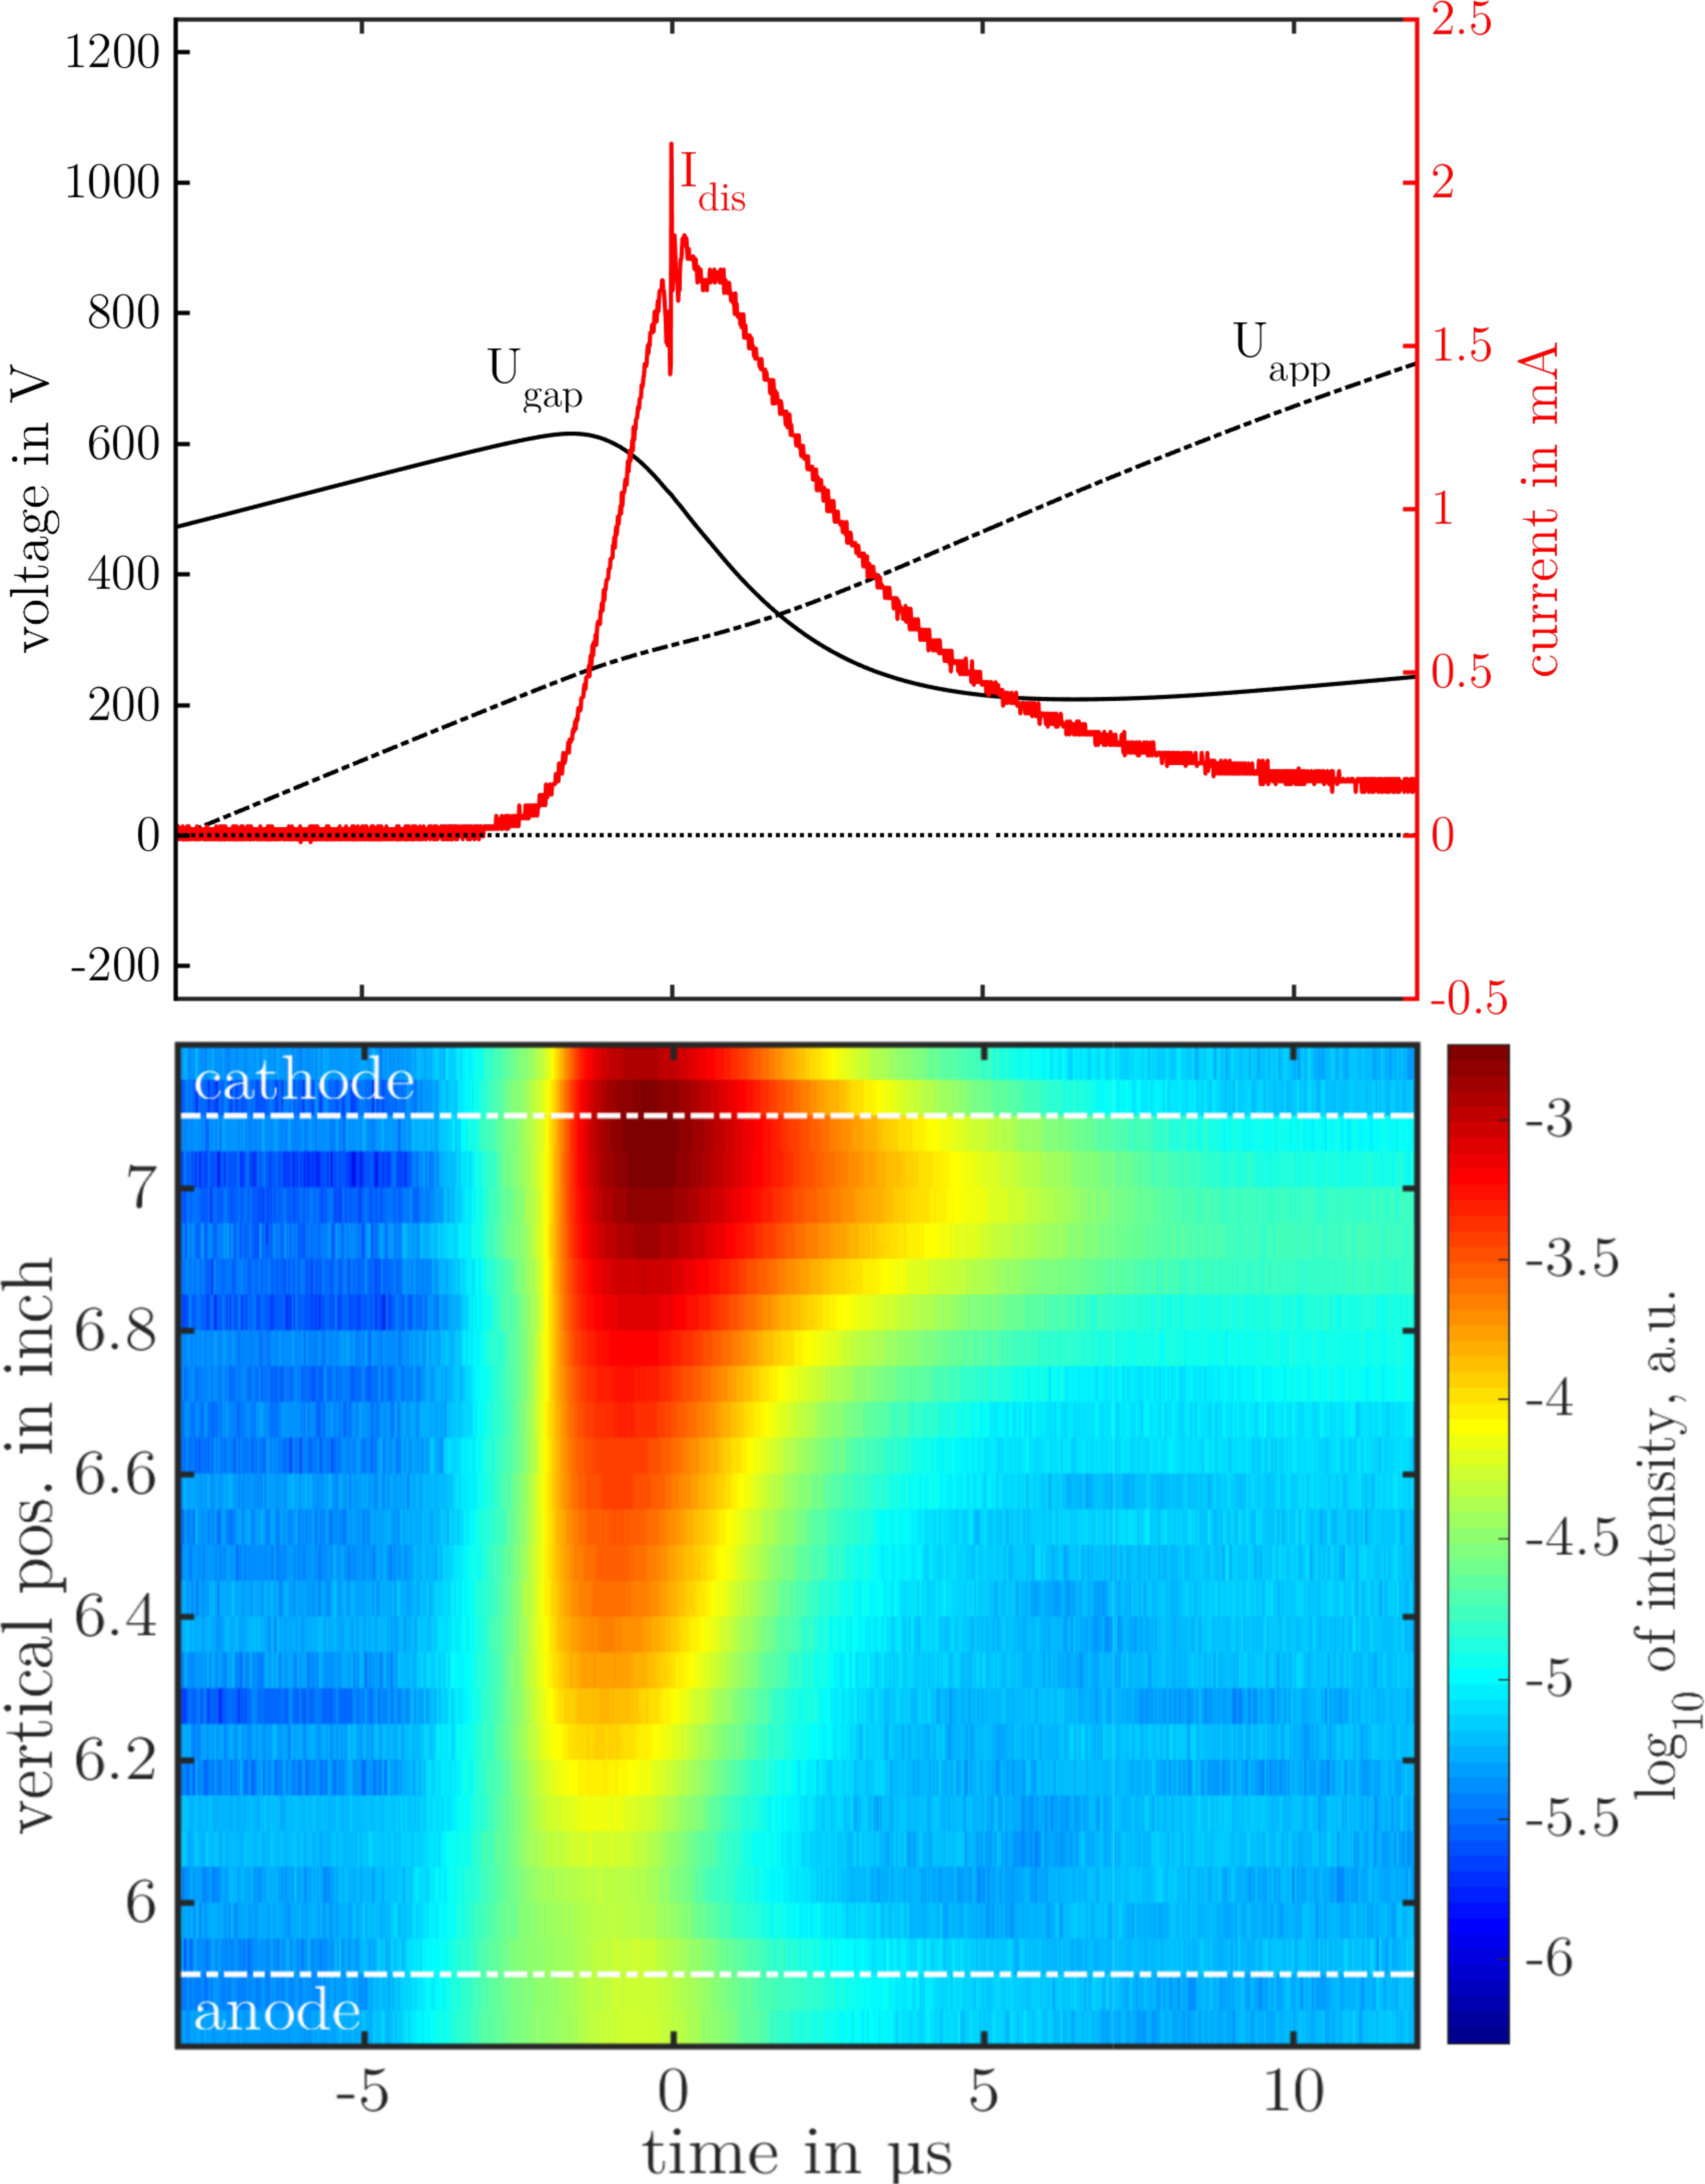
\includegraphics[width=\textwidth]{figures/706nm@sine/combination.pdf}
						\caption{}
						\label{img:combsine}
					\end{subfigure}
					\hfill
					\begin{subfigure}[t]{0.49\textwidth}
						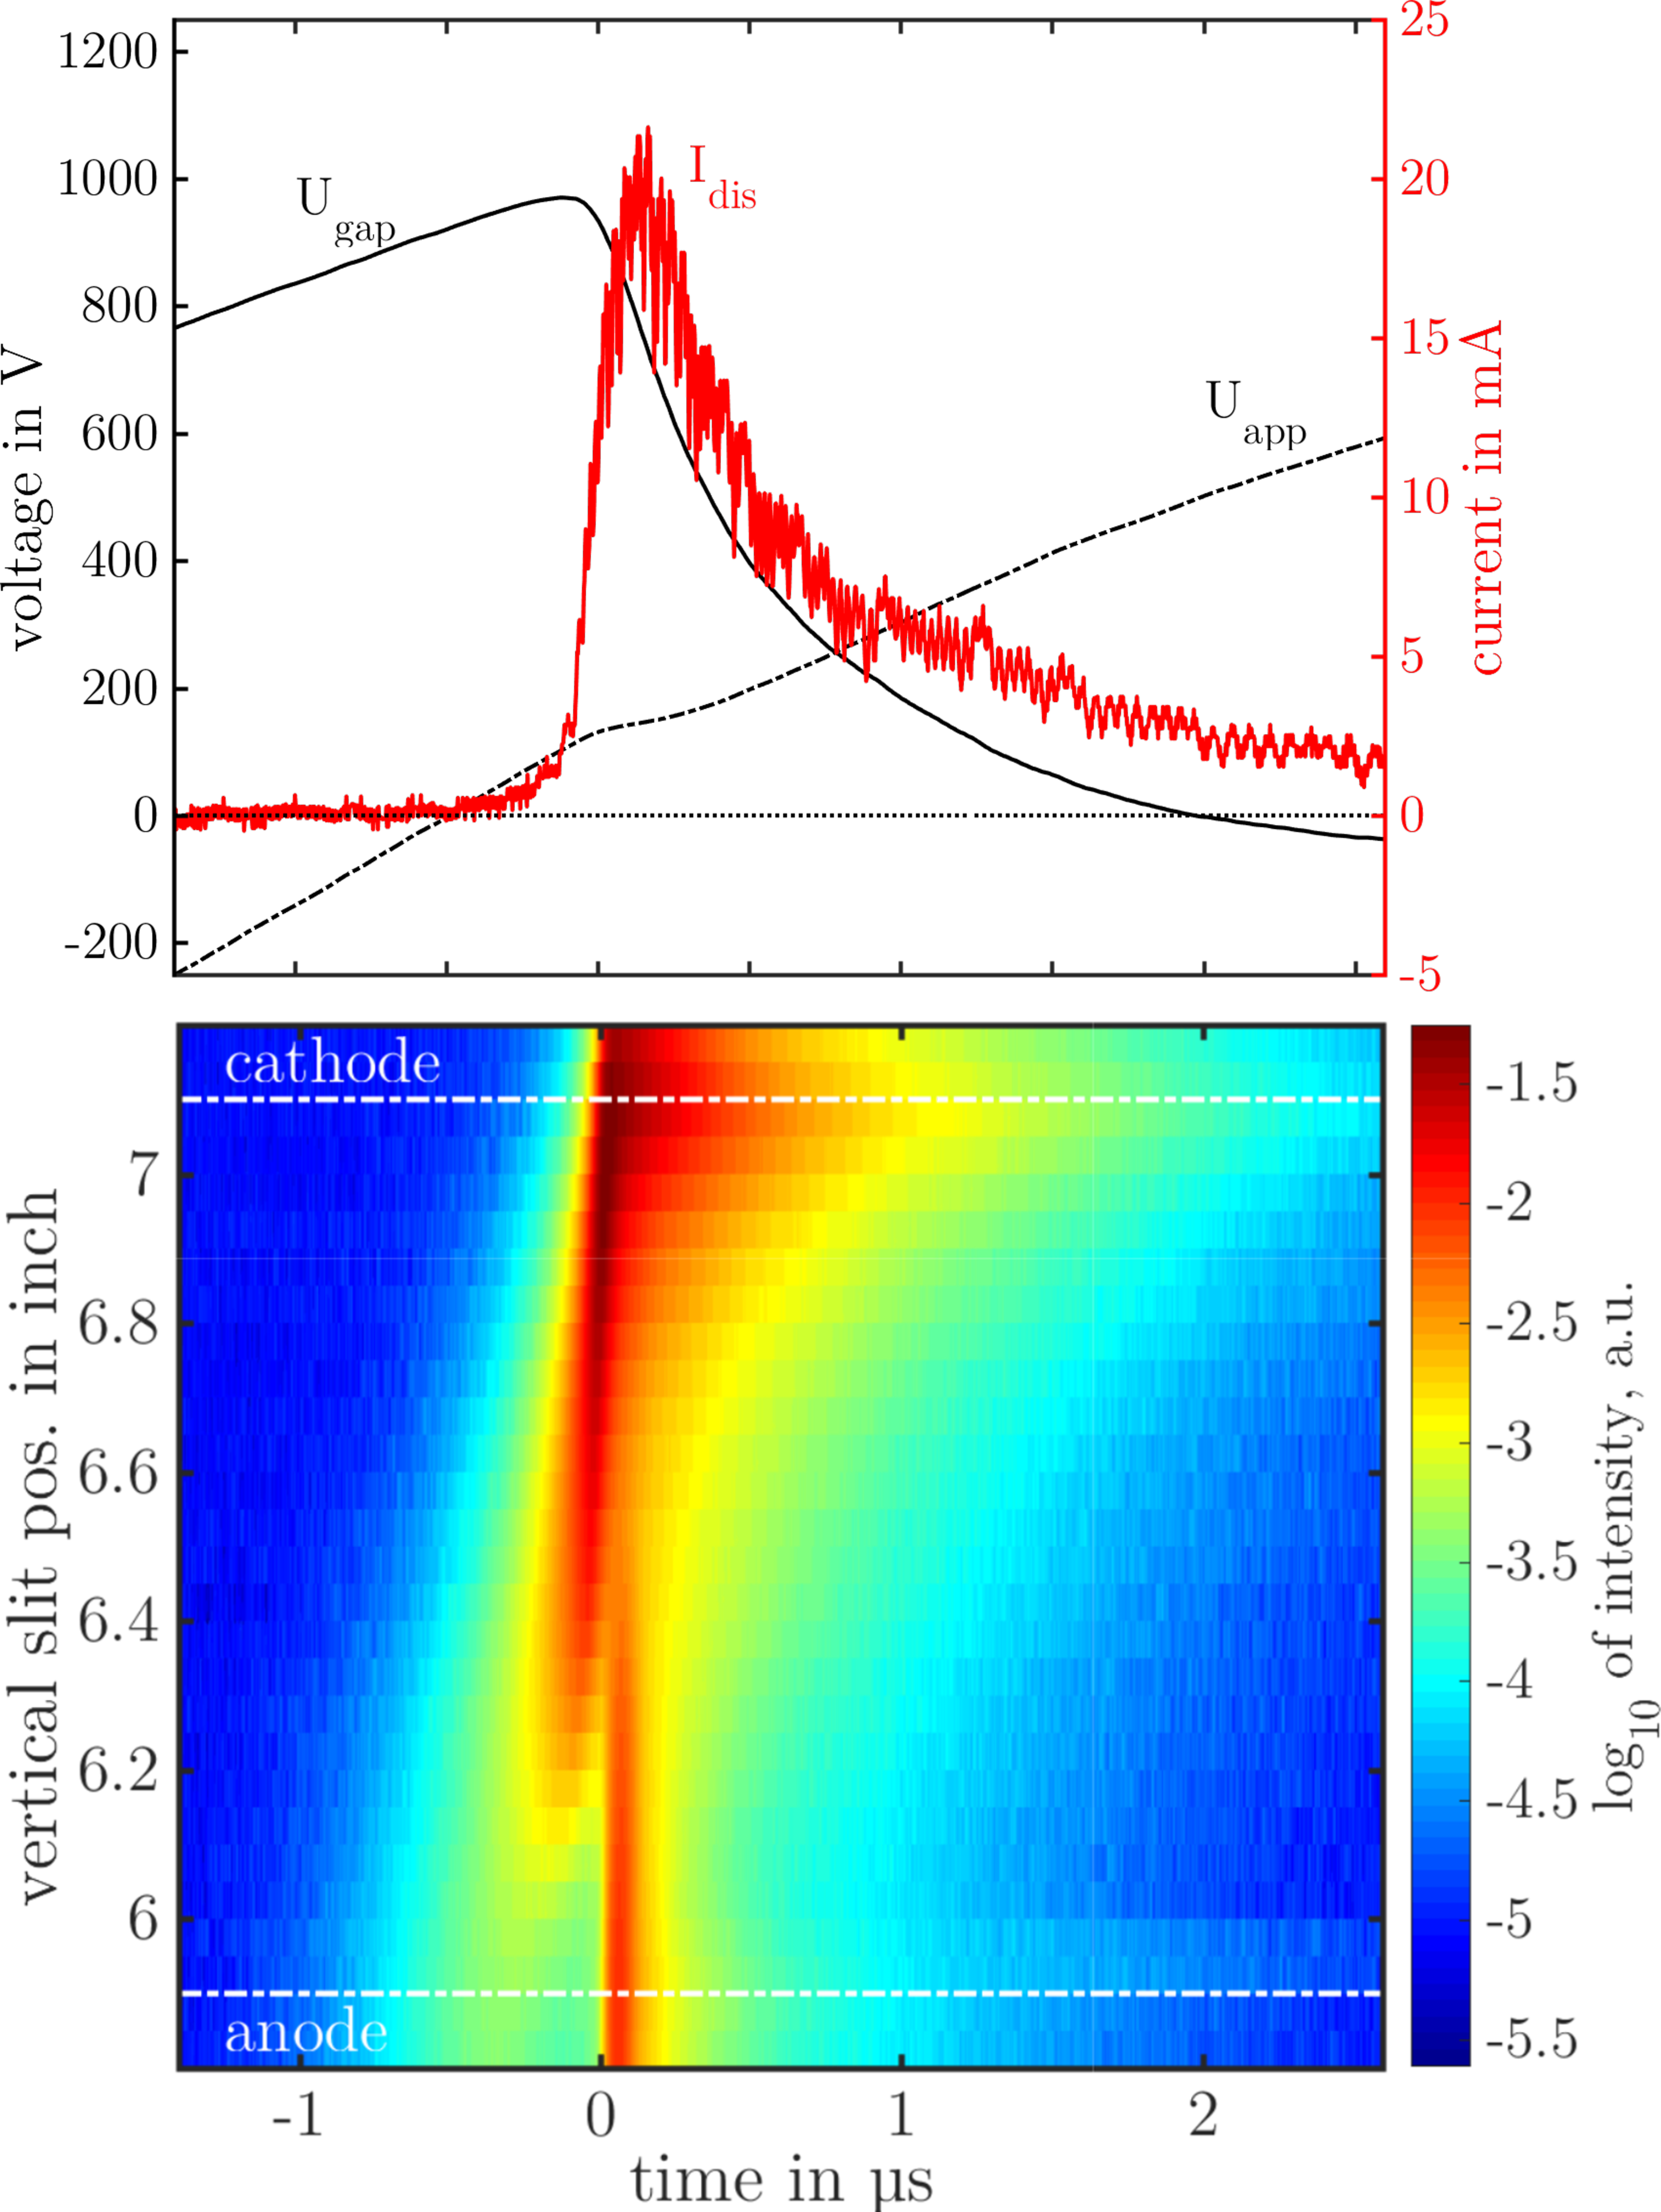
\includegraphics[width=\textwidth]{figures/706nm@square/combination.pdf}
						\caption{}
						\label{img:combsquare}
					\end{subfigure}
					\caption{Comparetive arrangement of spatio-temporally resolved emission profiles at $\unit[706,66]{nm}$ and discharge development for BDs excited by a \fett{(a)} sine, or \fett{(b)} square wave.}
					\label{img:comparisonsinesquare}
				\end{figure}
				
	\begin{multicols*}{2}
			
	\end{multicols*}
				
	\twocolumn

		The discharge currents $I\ix{dis}$ also differ by one oder of magnitude, as well as slope and width of the peak are not the same. This is due to a longer preliminary phase for an applied sinus wave voltage. A lower slope favors the accumulation of more volume charges, therefore the discharge is able to ignite at low breakdown voltages. Furthermore, the sine wave has a longer rising time, therefore the ions have more tome to travel to the cathode and induce secondary electrons from there.\\					
		Now that the development of the electrical properties for our presented BDs and the different applied voltages has been evaluated, the results have to be put in relation to the enclosed spatio-temporally resolved optical emission. The bottom of \autoref{img:combsine} and \autoref{img:combsquare} shows the temporal development of emission intensities at $\unit[706,66]{nm}$ between (dashed white lines) anode and cathode. Above/beyond one can see the reflection from the dielectric surfaces.\\
		During the preliminary Townsend phase, both voltage forms show weak emission in front of the anode, which indicates the starting exponential electron multiplication. Therefore, positive space charges are build up in front of the anode, since heavy ions are not as mobile as electrons. The resulting cathode-directed ionization front culminates in the breakdown, right when the maximum current is flowing (see \autoref{img:massines}). Fast electrons are rushing towards the anode, exciting and ionizing on their path. This causes an emission maximum, which increases over time in towards the cathode. Especially \autoref{img:combsquare} shows this very distinctively.\\
		Between this negative glow and the cathode, there is space charge with almost no electrons. The ions are accelerated here, like in a gravitational free fall. This cathode fall region yields a very high electric field and high ion density.\\
		An anode-sided counterpart of the negative glow, which consists of a spatially extended region with hight charge densities - see \autoref{img:massines}, is called positive column. This can only be seen at the emission profile of a square wave discharge. Here, the ionization front moves through the gap very fast. Quasi neutrality is almost satisfied, which means the electric field strength is low and constant. Only shortly before the positive electrode, inside the anode dark space, electron and ion density decrease. Hence, the emission is attenuated there.\\
		Further on in the temporal development of the discharge, emission is decreasing as excited species are relaxing. The breakdown removes a majority of free charges, which is why flowing current and glow diminish over time. Here, the maximum remains in front of the cathode. This afterglow is much wider and longer for a sine wave discharge, than for the square wave. This is due to the lesser slope in current, voltage and therefore slower charge transportation over the discharge volume.\\
		One should note here, that the gap voltage is not supposed to become negative throughout the discharge development, as this would invert charge flow. This is though shown in the top of \autoref{img:combsquare}. It has not become clear whatsoever, why this is the case here. 
		
	\subsection{Electric field strength measurement by He I line intensity ratios}
		
		After characterizing the discharges electrical properties and hence, the corresponding dynamics of the spectral emission, one will evaluate the full intensity profile for all four transitions mentioned above.\\
		Here, presented results have been received from the discharge of \autoref{img:combsquare}. Hence, this experiment has been executed at a square wave voltage of $\unit[1,2]{kV}$, $\unit[5]{kHz}$ and gas flow rates of $\unit[100]{sccm}$ He + $\unit[0,05]{sccm}$ N$_2$ at $\unit[1]{bar}$. A grating of $\unit[1800]{mm^-1}$ and MC entrance slit height and width of $\unit[0,2]{mm}$ and $\unit[1]{mm}$, respectively, was chosen. Additionally, the OG1 filter remains in the optical path.\\
		Results are shown in \autoref{img:667u728nm} and \autoref{img:706u587nm}. The $\log\ix{10}$ of all four profiles shows the same trend, whereas the transition $3^3$S-$2^3$P yields intensities one order of magnitude higher than the rest. Also, areas with values of $\tenpo{-2}$ and higher are much broader than, for example at $\unit[667,98]{nm}$. The remaining three, less intense emission profiles for singlet and triplet have about the same order of magnitude for maximum and minimum. Again, slight differences in temporal extend can be seen between the singlet and triplet emissions, as the latter happen to be a little wider.\\
		As shown \cite{linratio1_14}, \cite{lineratio2_14} and discussed in the previous sections, the local electric field strength in helium BDs at elevated pressures is, to some extend, related to the optical emission of excited singlet and/or triplet states. Therefore, one would expect to find similar intensity profiles for singlet and for triplet transitions respectively, as they should be de-/populated by the same processes. And indeed, this is the case for $\unit[667,98]{nm}$ and $\unit[728,31]{nm}$. Here, the upper states are predominantly populated by electron impact, therefore making them good candidates for field strength measurements, as they almost solely depend on the production of energetic electrons. It is also shown in \cite{linratio1_14}, \cite{belmonte}, \cite{debreuil} that the main mechanism, which dominates the populations, is the difference in excitation rates for $3^1$D, $3^1$S and $3^1$P levels, which is very effectively transferred to $3^1$D via excitation transfer - see \autoref{img:termnschema}. The fast decay of intensity after the discharge breakdown indicates the depopulation, mainly through spontaneous emission, as the mean lifetime is in the nanosecond range \cite{linratio1_14}. Thus it is found, that both profiles are directly influenced by electron temperature. This is also taking into account, that a faster decay in intensity than discharge current indicates such relation \cite{electron_temp}.\\
		In comparison to the triplet transitions, the temporal extend of given emissions in \autoref{img:706u587nm} is between $\unit[0,2]{\upmu s}$ ($3^3$S-$2^3$P) and $\unit[0,7]{\upmu s}$ ($3^3$D-$2^3$P) longer, than those of the singlet states. Hence, de-/populating processes with such rates have to contribute only to those intensities. And indeed, it was already discussed that triplet line emission is strongly affected by metastable densities. Furthermore, the excitation from $2^1$S to triplet states is orders of magnitude more probable, than vice versa, contributing to such intensity profiles. Hence, emission from excited triplet states is much higher.\\
		Overall, all four line intensity profiles show the characteristic temporal development of the ionization front towards the cathode, as well as increasing after glow in high field regions near the negative electrode and a positive column. Other than that, the Townsend phase is clearly distinguishable in front of the anode. At $\unit[706,66]{nm}$, the spatially further extended ionization front already interferes with this phenomenon. Thus it could be concluded, that the metastable density benefits from the developing ionization front, reinforcing emission from $3^3$S. And again, in \cite{linratio1_14} it is mentioned, that for electric field strength values below $\unit[4]{kV/cm}$, excitation from metastable levels becomes significant, which also contributes to the emission early on in the discharge.\\
		After discussing the individual transitions, line intensity ratios can be calculated from given results. The quotient between the intensities of the singlet and triplet states, respectively, is calculated and shown in \autoref{img:comparisonlineratio}. Here, the quantities are denoted as $R\ix{sing}=I\ix{667}/I\ix{728}$ and $R\ix{trip}=I\ix{706}/I\ix{587}$. Due to the low field values during the preliminary phase of the discharge and diminishing intensities, experimental determination of emission was difficult. Hence, numerical calculation of quotients from values as small as $\tenpo{-6}$ was not pursued. Therefore, intensities of up to 5\% off the maximum have been exclude and set to zero for each line emission.\\
		As seen for $R\ix{sing}$ in the top of \autoref{img:comparisonlineratio}, the ratio has its maximum of around 2,2 in front of the cathode, decreasing along the trend of the ionization front towards the anode. Inside the positive column during the breakdown, $R\ix{sing}$ is around 1, meaning that populations and the corresponding processes are in some equilibrium for $3^1$S and $3^1$D. Later on in the discharge, the intensity ratio decreases slowly. Hence, in the afterglow, emission from $\unit[667,98]{nm}$ is more attenuated than its counterpart at $\unit[728,31]{nm}$.\\
		The line intensity ratio in \autoref{img:comparisonlineratio} for the triplet states (bottom) shows a quite different behavior. Here, one finds a much higher maximum at around 14, which is located in the transition between positive column and ionization front. Other than that, the whole positive column carries a high ratio of 12 and more, whereas afterglow, cathode fall and negative glow in front of the upper electrode only reach up to 7. The ratio even decreases to 5 during the breakdown in front of the cathode and remains so.\\
		In \cite{Massines}, \cite{0022-3727-36-1-306} a theoretically calculated electric field strength - spatio-temporally resolved in \autoref{img:massines} - and densities - between anode and cathode in \autoref{img:golubovskii} - have been achieved. The trend of the local field strength and electron density in Massines' et al. calculations shows, that inside the positive column low excitation rates and energies can be expected, therefore leaving the intensity ratio at around 1 as both states are populated equally. Further on in the discharges development towards the cathode, electron energy - with corresponding electric field - and counts increase dramatically, which is why impact ionization of the energetically higher state is preferred. Hence, the ratio rises and reaches its maximum during the discharge breakdown in front of the negative electrode. Any decrease afterwards is a result to the relief of charges during the breakdown, reducing field strength and densities. Thus, the population of higher states diminishes faster, because remaining electrons might not carry the necessary kinetic energy anymore.\\
		Applying said theoretical results to the figure for $R\ix{trip}$, it becomes obvious why the ratio shows such a different behavior: when the local field strength, therefore electron energy and density is low, metastable populations significantly influence the excitation rates for $3^3$S. During the Townsend phase and the development of an ionization front, solely the energy of metastable levels is sufficient for electronic excitation from the ground state. As the intensity ratio decreases towards the cathode, the lower $3^3$D level benefits from an increase in electron number, hence $R\ix{trip}$ is reduced. Overall, the emission at $\unit[706,66]{nm}$ is much higher because of the effective excitation transition from singlet ground states $2^1$S.\\
		Finally, after evaluation of given line intensity ratios with respect to density and electric field development, one can utilize a collisional-radiative model for singlet transitions \cite{linratio1_14} to quantify such field strength. If all of the above mentioned effects are taken into account, a fourth-order polynomial can be acquired:
		
			\begin{align}
				E\ix{LR}\left[\frac{kV}{cm}\right] =\,\, &2,224-20,18R\ix{sing}+45,07R\ix{sing}^2 \nonumber \\ 
				&-19,98R\ix{sing}^3+3,369R\ix{sing}^4\,\,. \label{eq:elfield}
			\end{align}
				
		This equation can be used, according to Ivkovi{\'c} et al. \cite{linratio1_14}, for calculations of electric fields in the range $\unit[3-40]{kV/cm}$ at atmospheric pressures and $\unit[310]{K}$. Again, an uncertainty between 1,5\% and 10\% is claimed. The result is shown in \autoref{img:elfield667}.\\
		Comparing the achieved values to the results of Golubovskii et al. \cite{0022-3727-36-1-306} in \autoref{img:golubovskii}, one finds great agreement for the spatio-temporal development. A maximum field strength is reached in front of the cathode during the discharge breakdown. Also, the ionization front is characterized by an increasing field towards the upper electrode, as one would have expected. Inside the positive column, densities and therefore electric field are low and constant. Also, very small values are calculated for areas between the positive column and near the negative glow and cathode fall region, whereas this is also found in \autoref{img:massines} and \autoref{img:golubovskii}. This is because of strong local space charges, compensating the applied electric field.\\
		The temporal evolution of the field strength shows great gradients towards its maximum and breakdown, but not in the afterglow. This might be due to the fast advance in exponential ionization until the breakdown voltage is applied and accumulated charges are drained by the discharge current. If the resulting quantities in field strength are indeed realistic has to be verified, e.g. stark spectroscopy.
		
	\onecolumn
			
			\begin{figure}
				\centering
				\begin{subfigure}[t]{0.49\textwidth}
					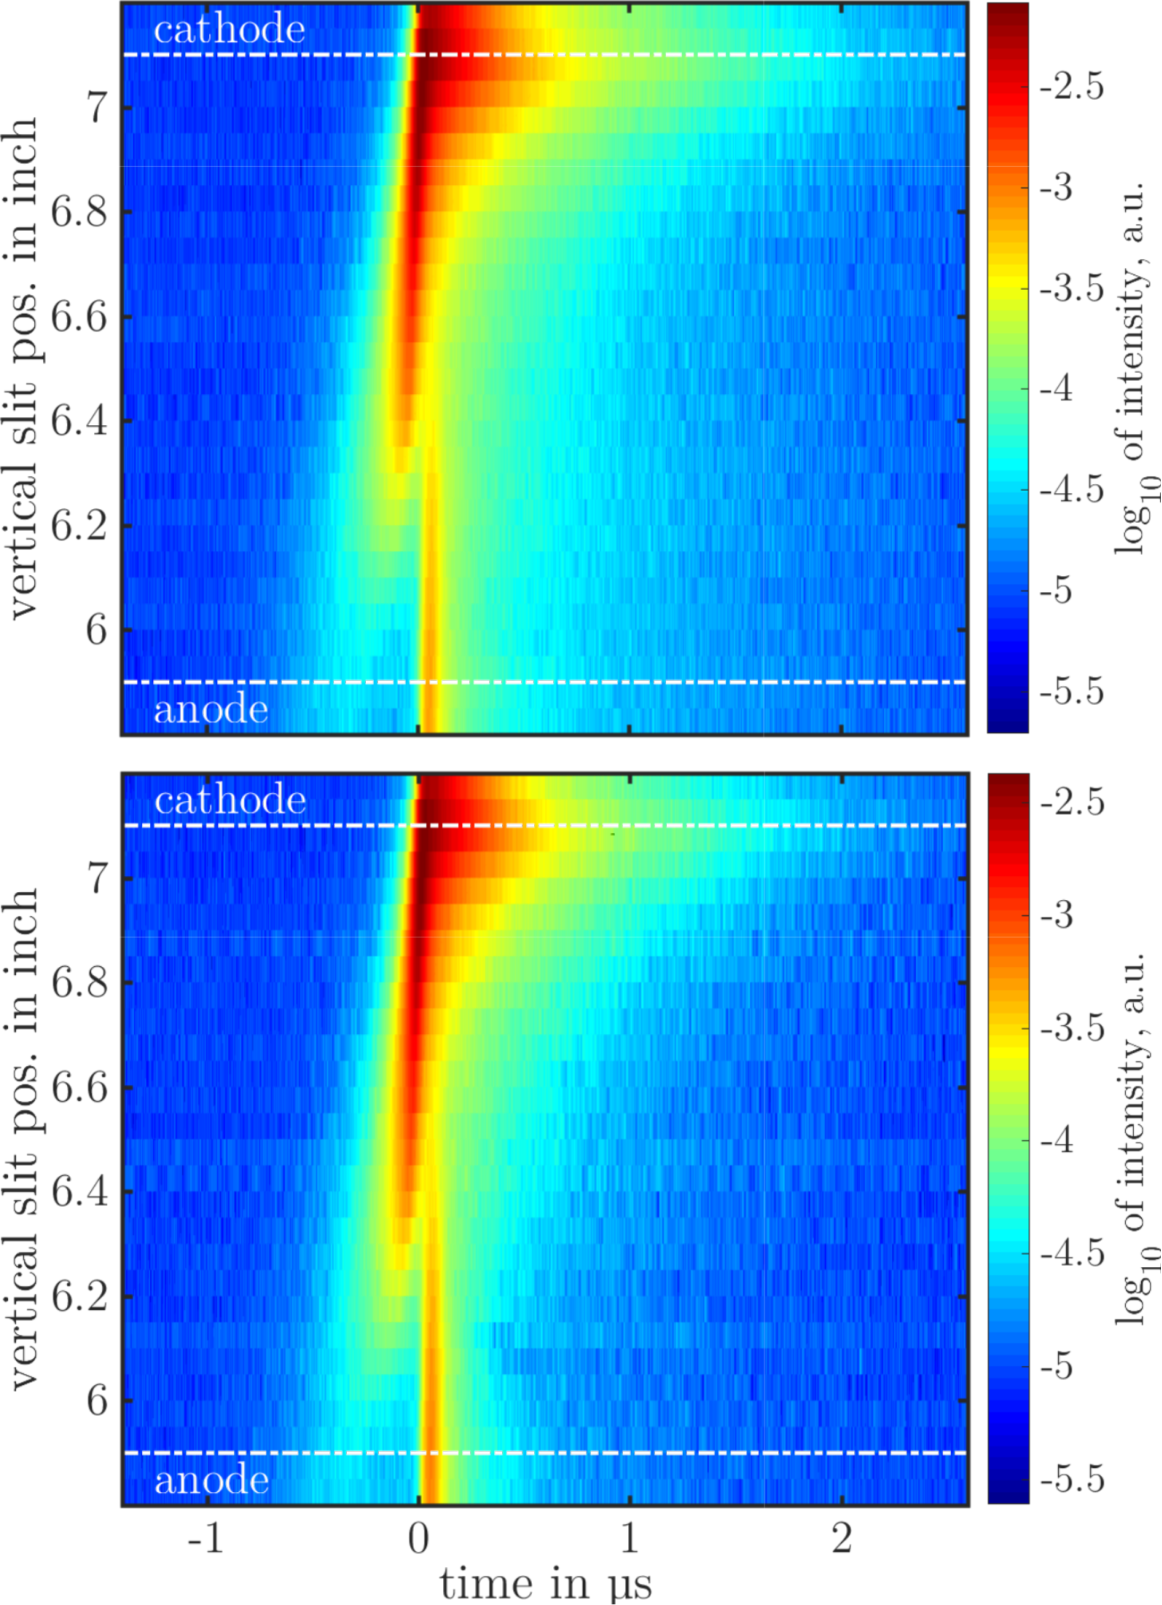
\includegraphics[width=\textwidth]{figures/lineratio/combinations/korr667over728.pdf}
					\caption{}
					\label{img:667u728nm}
				\end{subfigure}
				\hfill
				\begin{subfigure}[t]{0.49\textwidth}
					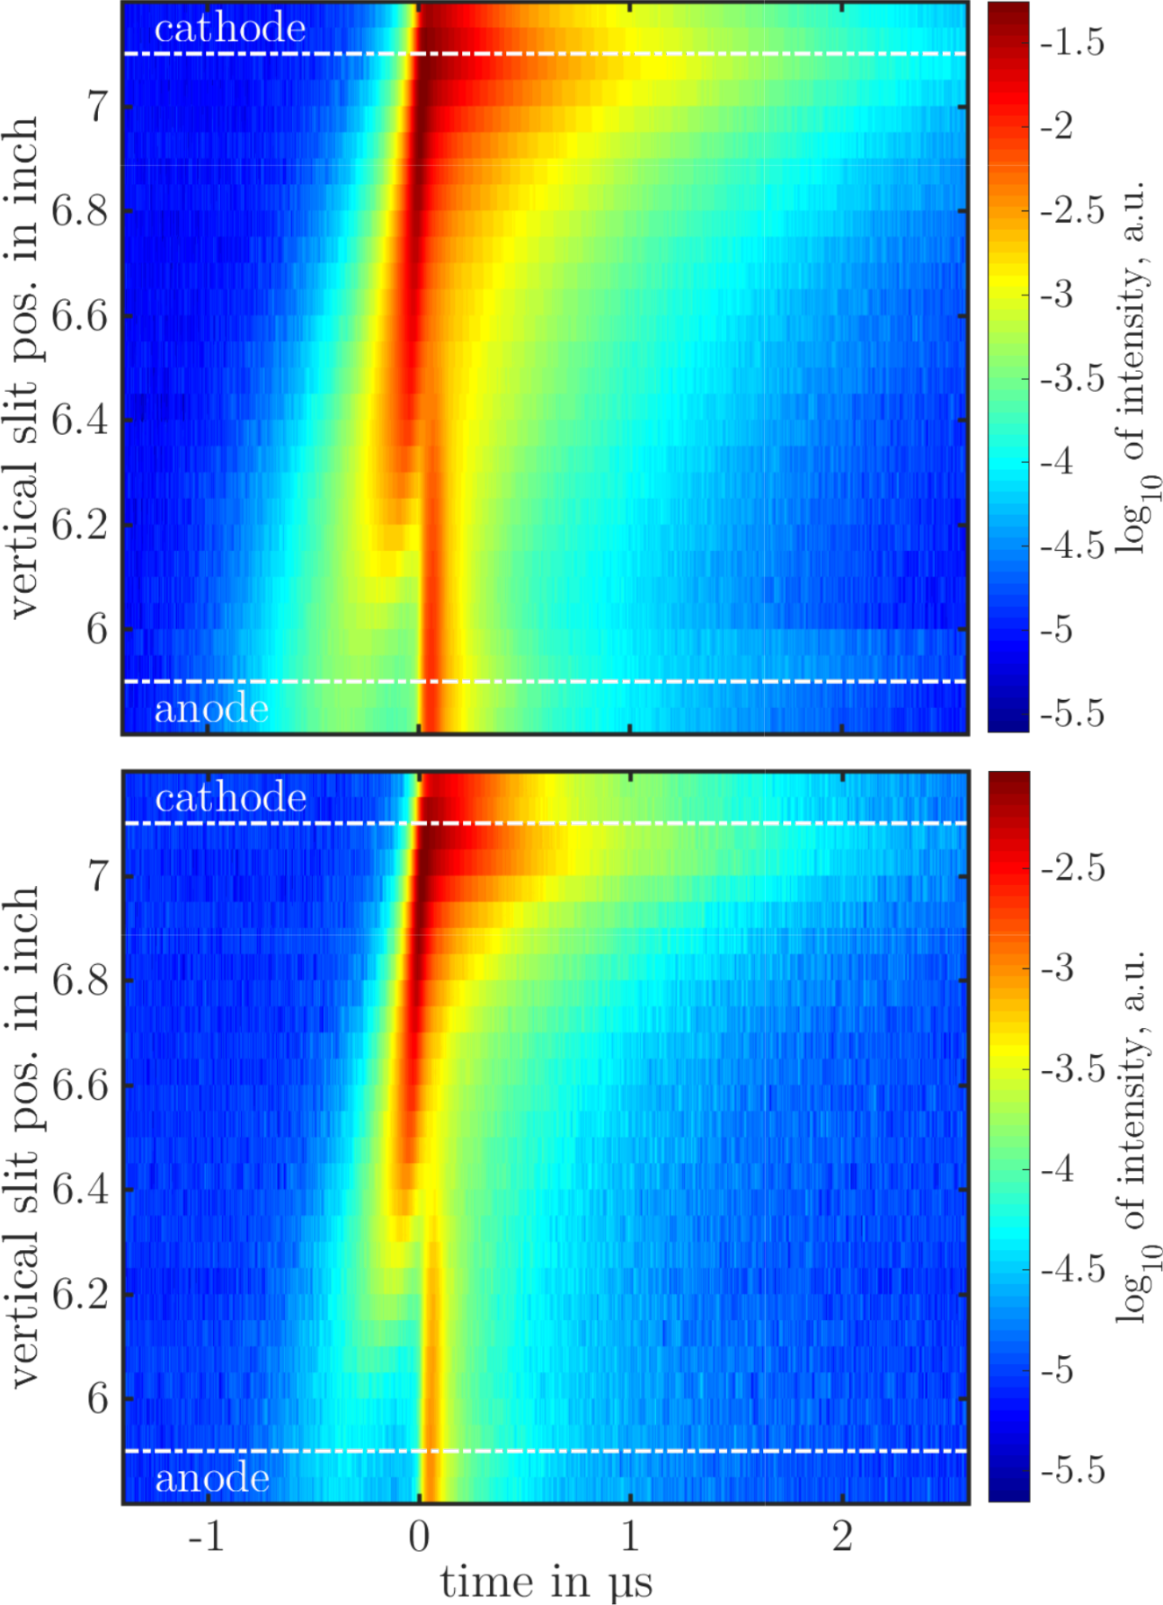
\includegraphics[width=\textwidth]{figures/lineratio/combinations/korr706over587.pdf}
					\caption{}
					\label{img:706u587nm}
				\end{subfigure}
				\vspace{0.3cm}
				\caption{\fett{(a)}: Spatio-temporally resolved line emission profiles for $\unit[667,98]{nm}$ (top) and $\unit[728,31]{nm}$ (bottom). \fett{(b)}: At $\unit[706,66]{nm}$ (top) and $\unit[587,65]{nm}$ (bottom).}
				\label{img:comparisonemissionline}
			\end{figure}
			
		\begin{multicols*}{2}
			
		\end{multicols*}
			
			\twocolumn
		
				\begin{figure}
					\centering
					\hspace{-0.5cm}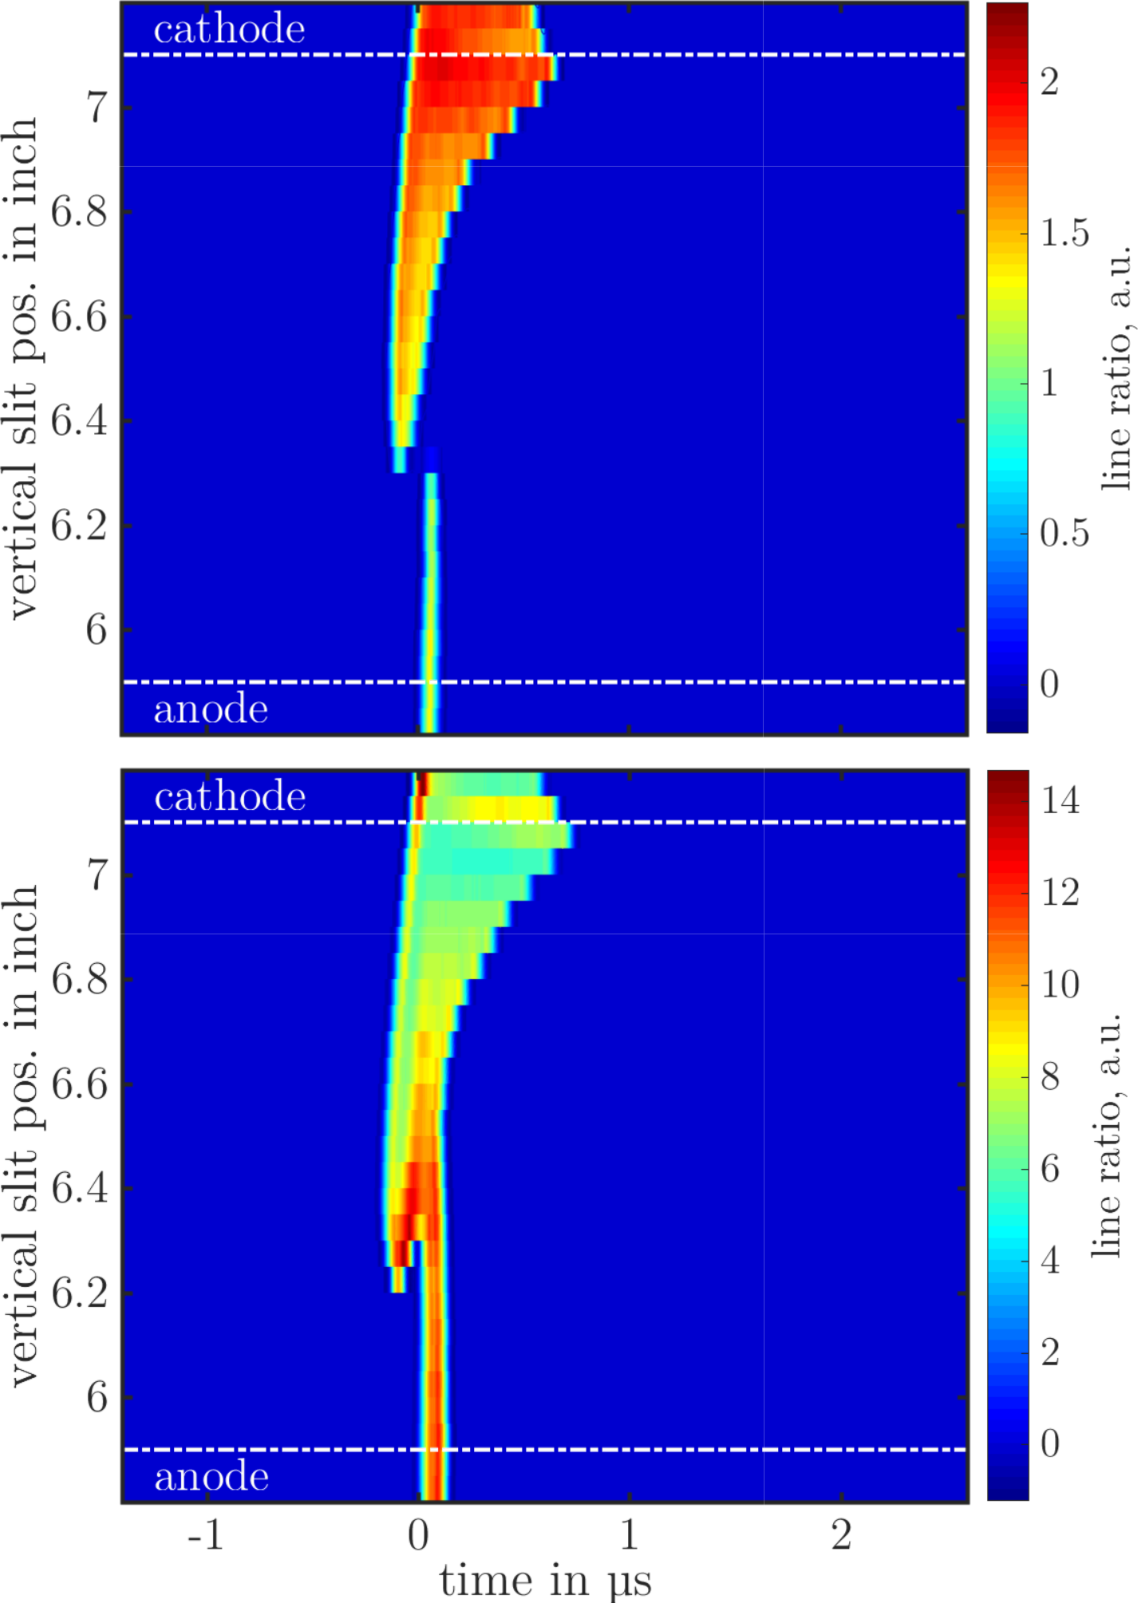
\includegraphics[width=0.5\textwidth]{figures/lineratio/combinations/lineratio667over706.pdf}
					\caption{Comparison of line emission ratios between singlet lines at the top and triplet at the bottom.}
					\label{img:comparisonlineratio}
				\end{figure}
				
				\begin{figure}
					\centering
					\hspace{0.5cm}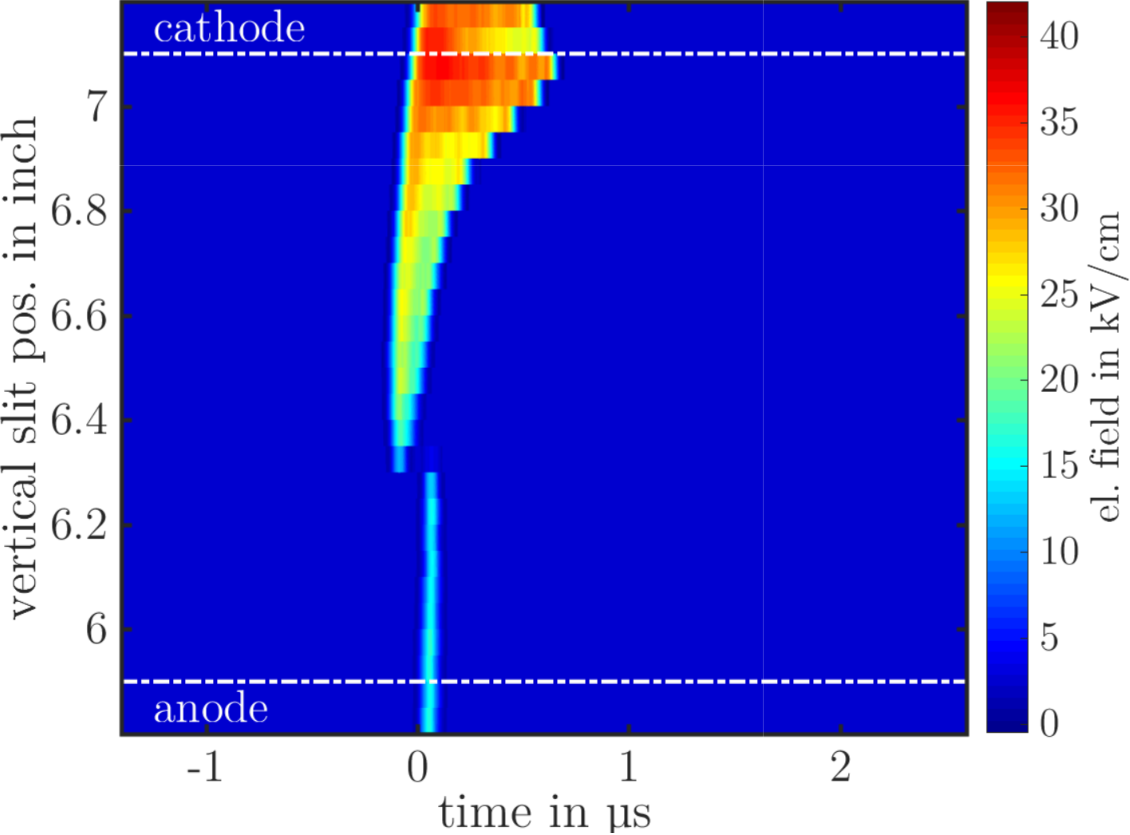
\includegraphics[width=0.5\textwidth]{figures/lineratio/combinations/electricfield667.pdf}
					\caption{Electric field strength between anode and cathode in a He+N$_2$ BD at atmospheric pressure. Calculated via \autoref{eq:elfield} from \cite{linratio1_14}.}
					\label{img:elfield667}
				\end{figure}
		
				\begin{figure}
					\centering
					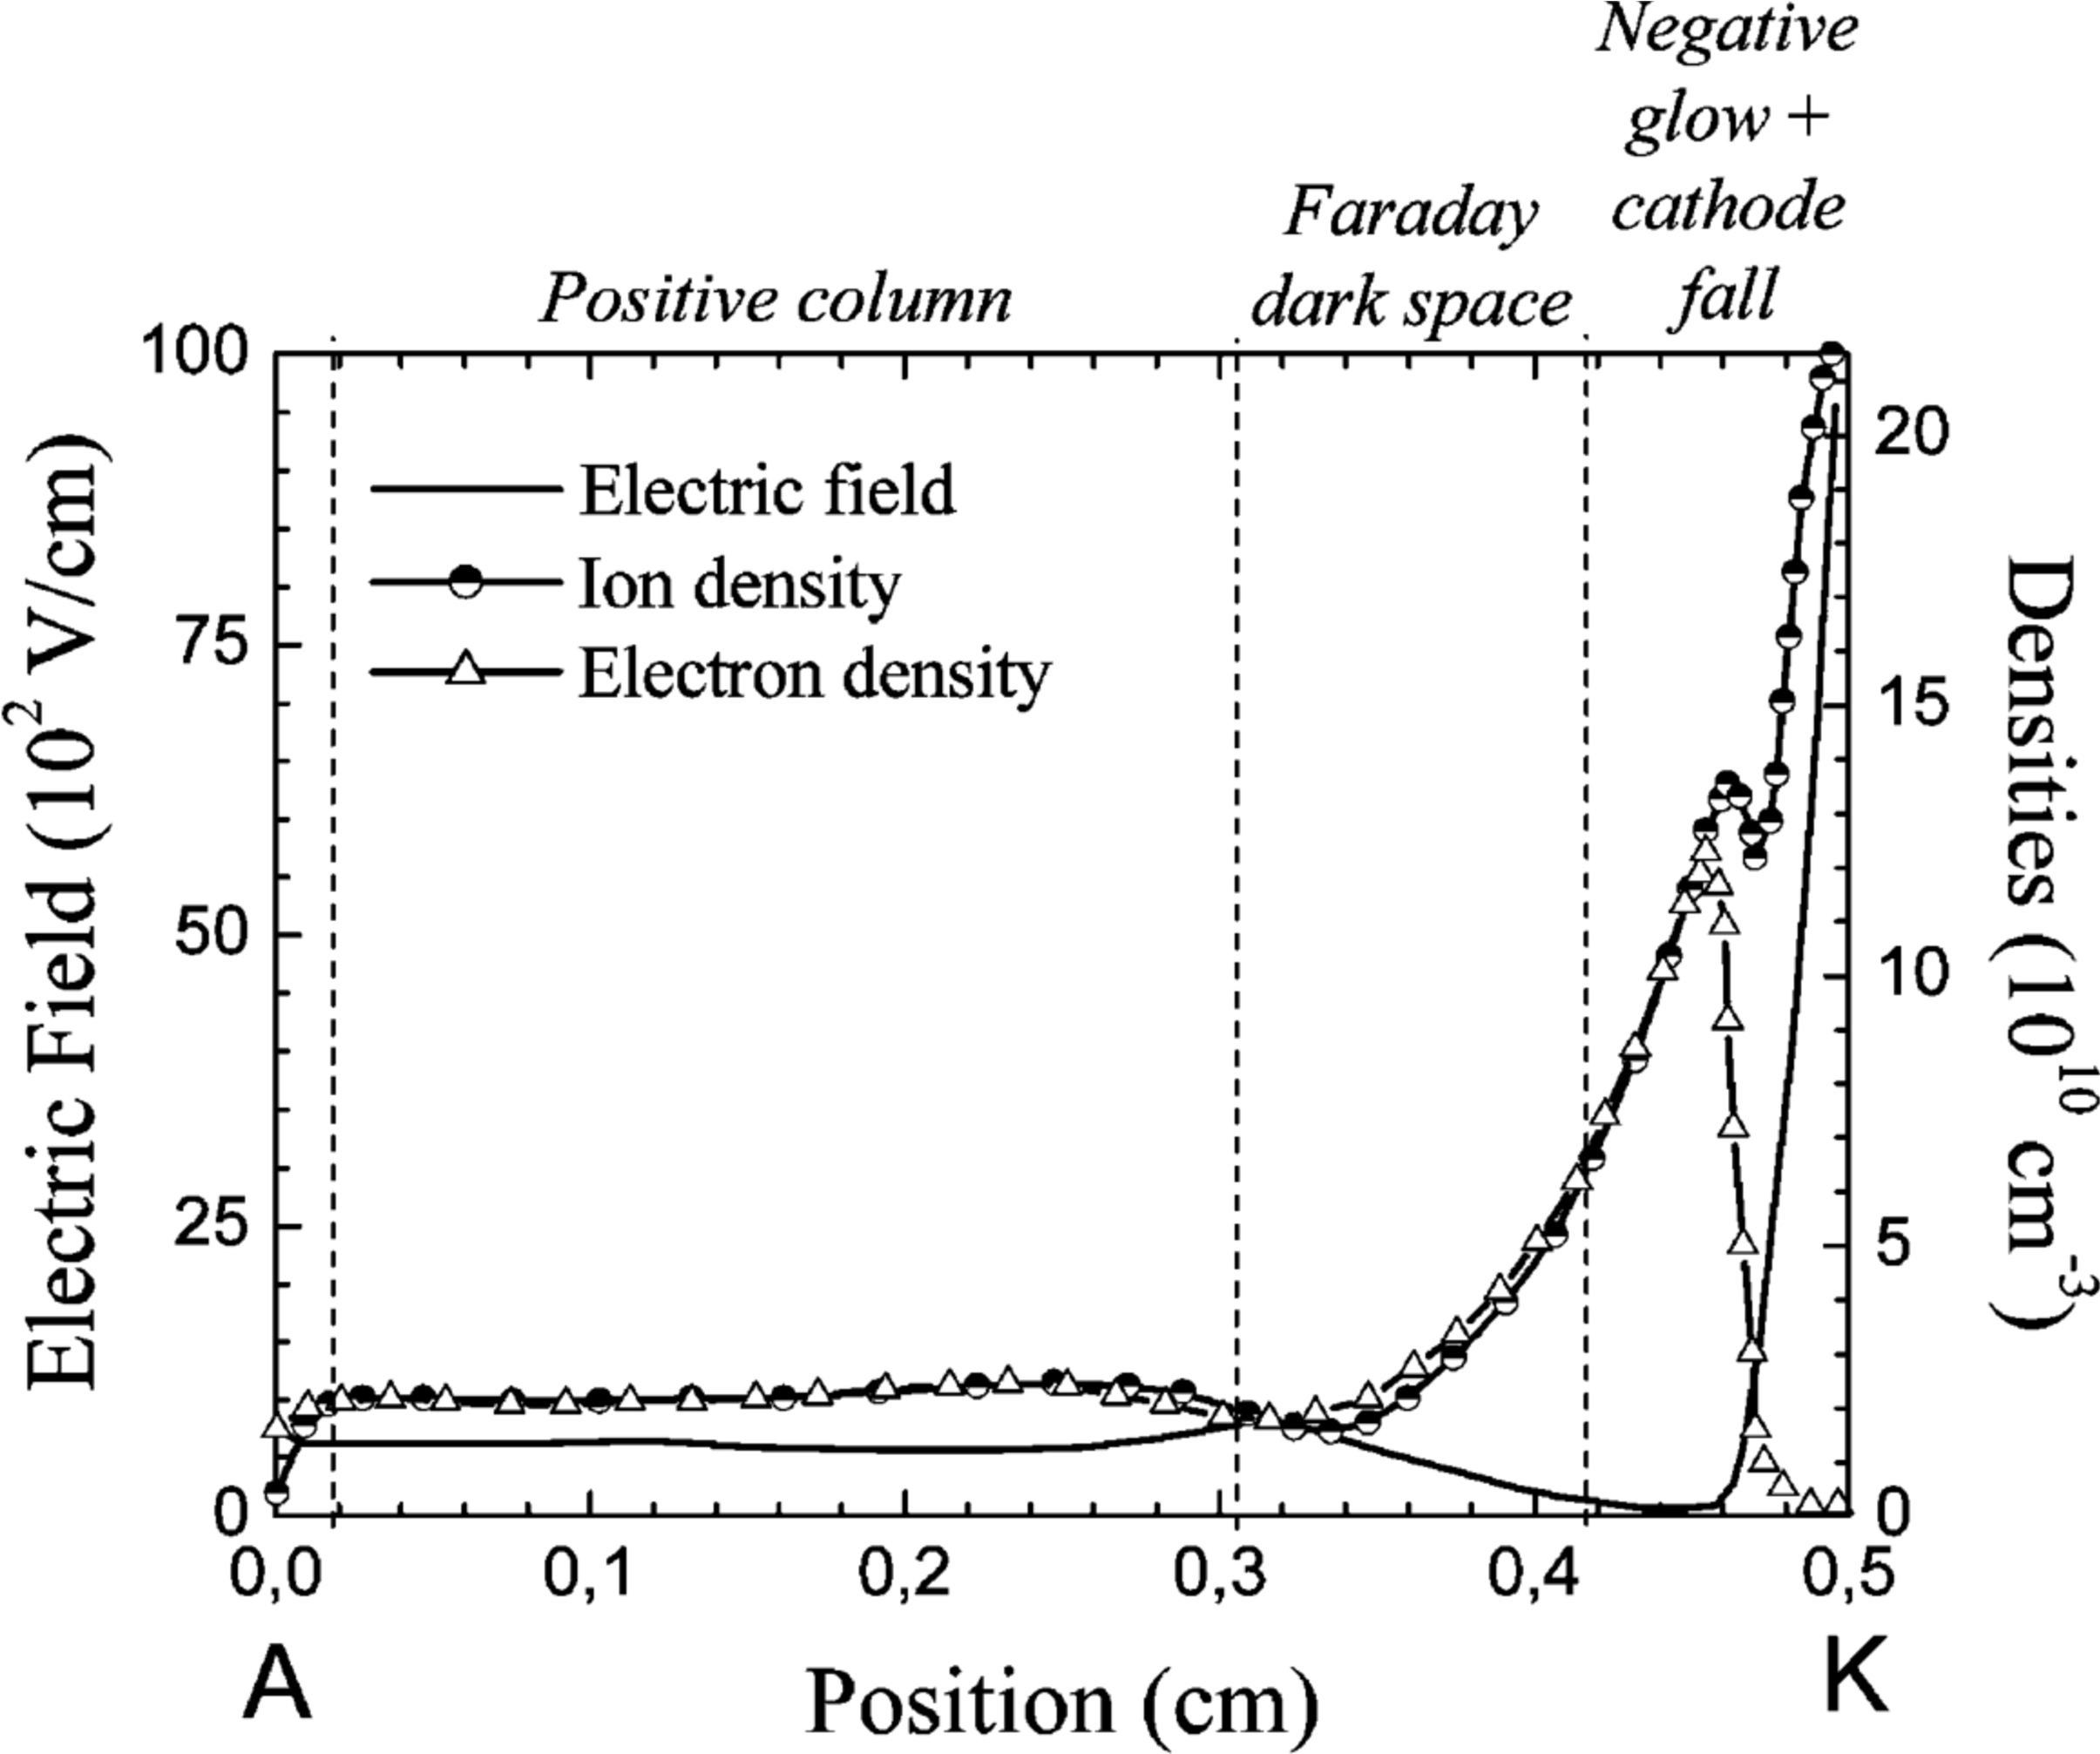
\includegraphics[width=0.5\textwidth]{figures/lineratio/massinesp3fig5.pdf}
					\caption{Calculated space distribution from the anode to the cathode of	the electrical field, the ion and electron densities in a He glow dielectric barrier discharge when the discharge current intensity is maximum. \cite{Massines}}
					\label{img:massines}
				\end{figure}
		
				\begin{figure}
					\centering
					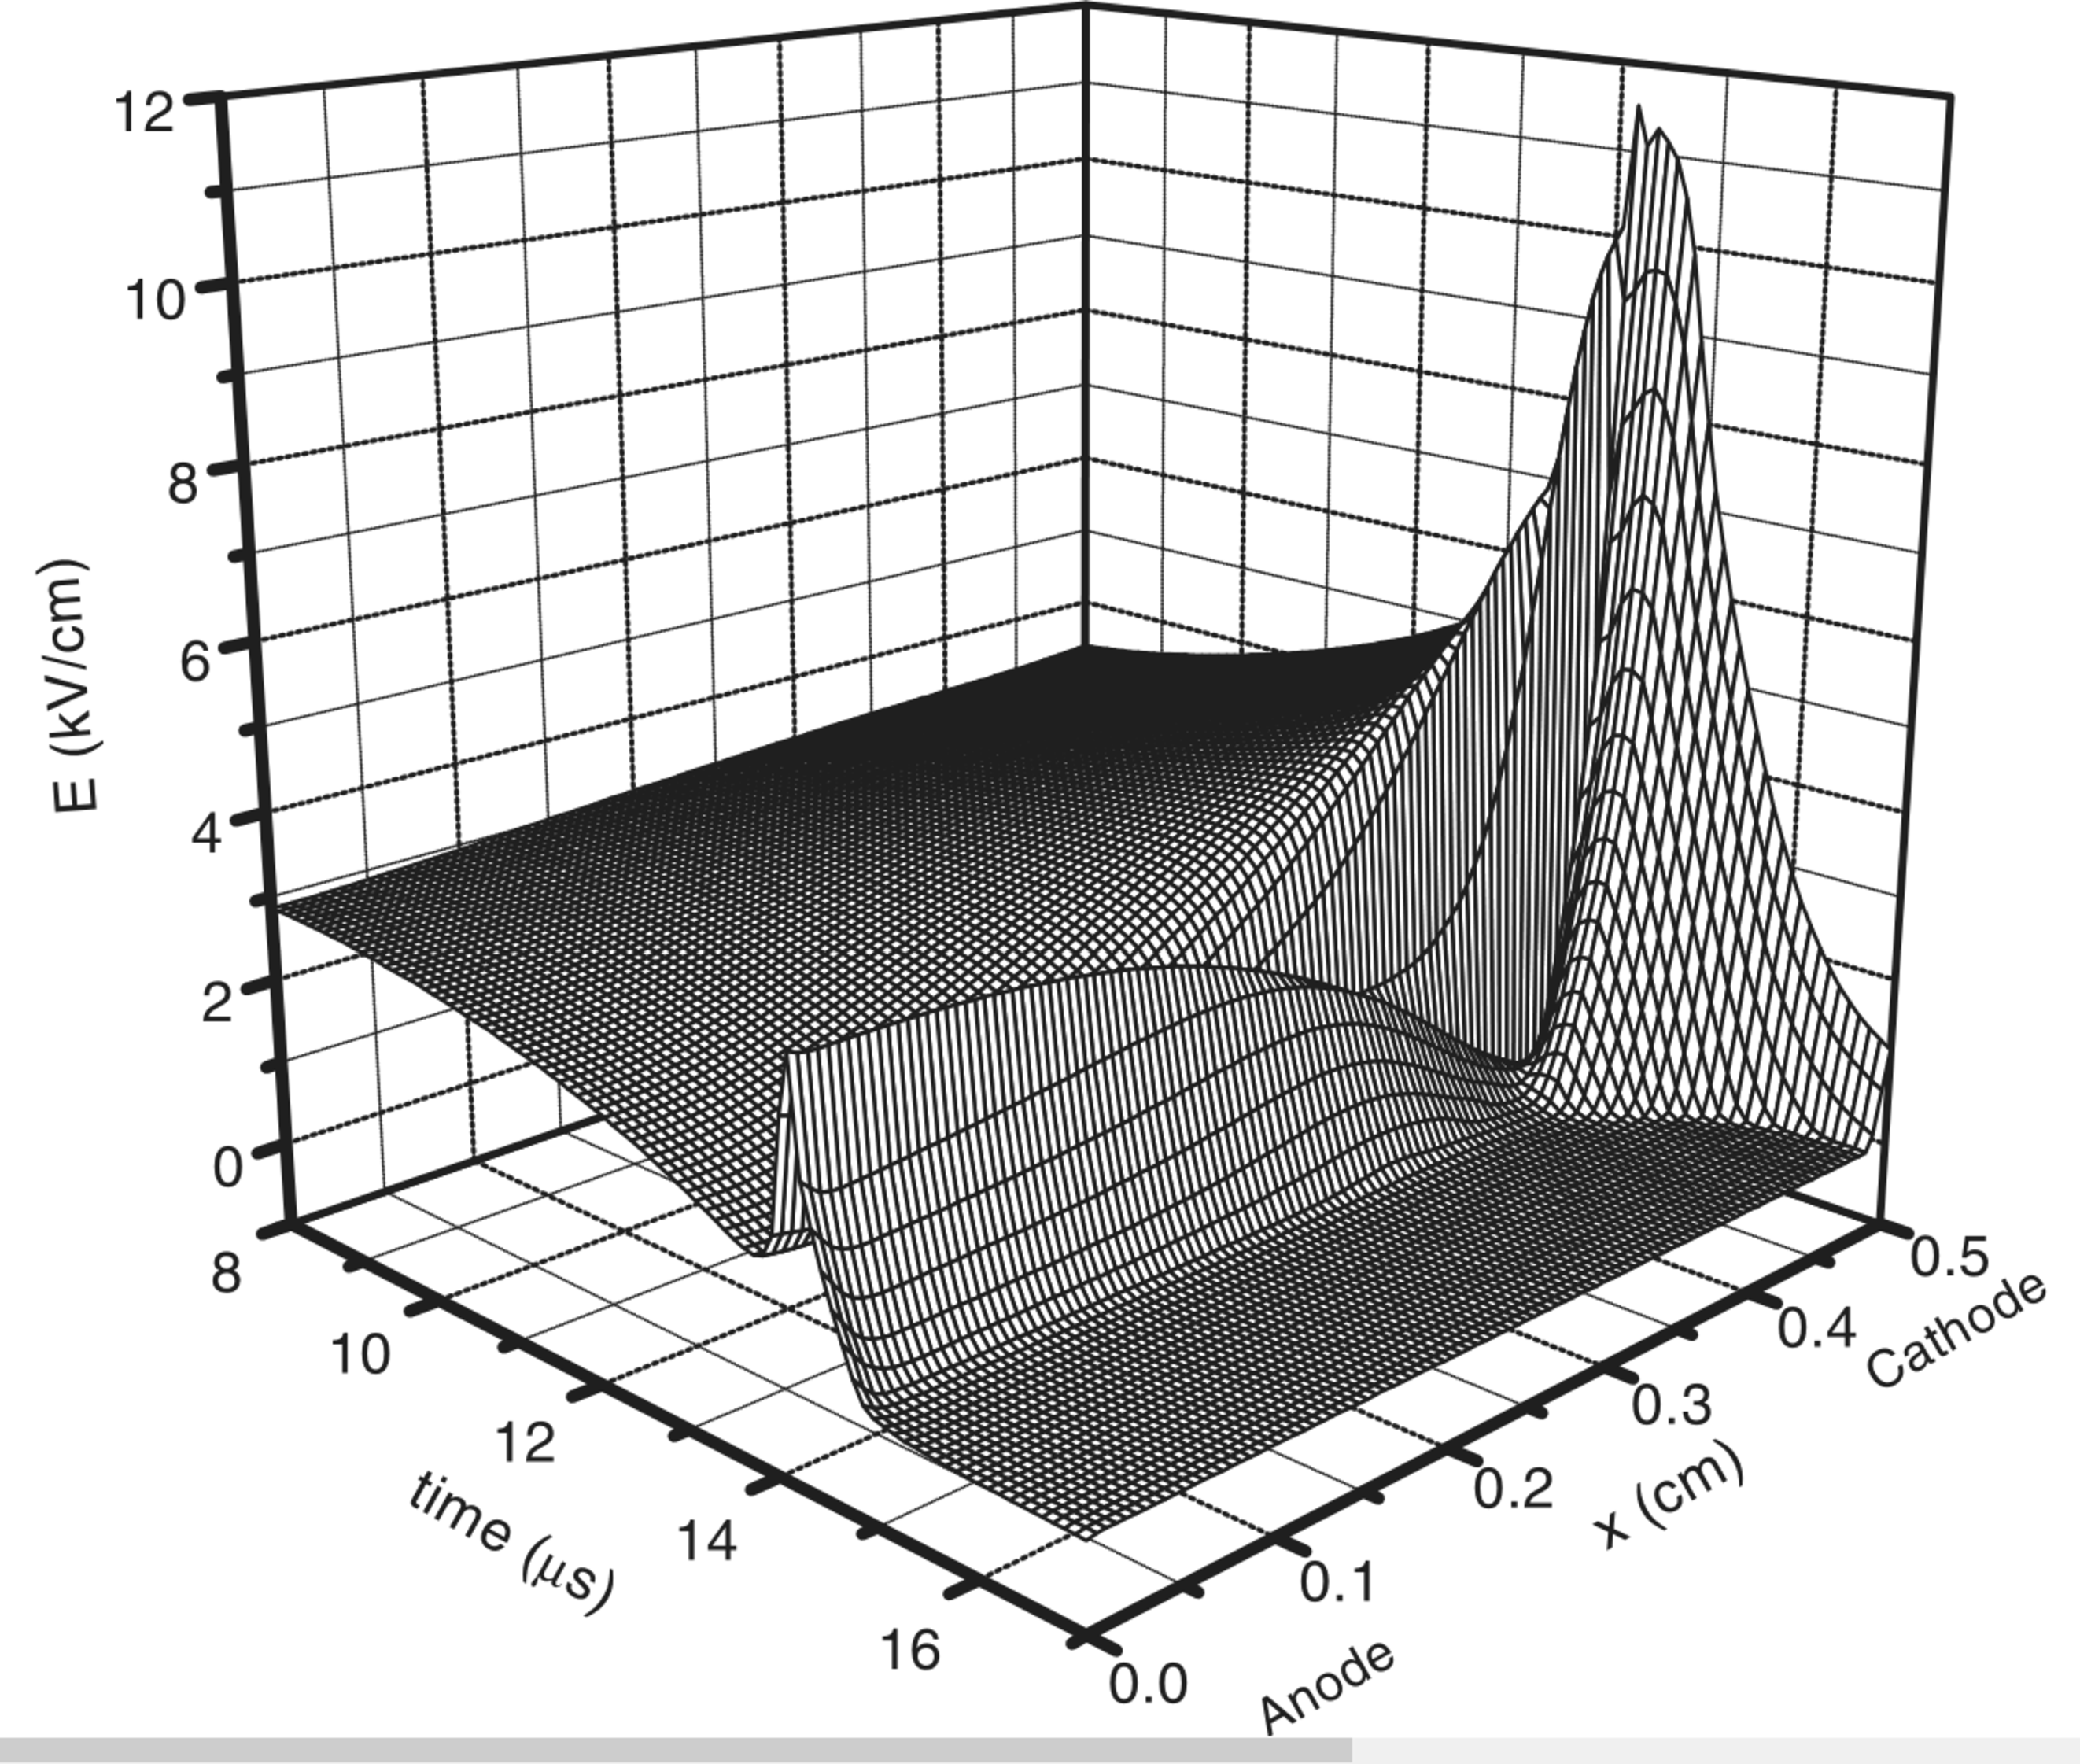
\includegraphics[width=0.5\textwidth]{figures/lineratio/golubovskiip47fig9}
					\caption{Three-dimensional plot of the electric field strength in the breakdown phase of glow discharge. \cite{0022-3727-36-1-306}}
					\label{img:golubovskii}
				\end{figure}
				
		\subsection{Electric field strength measurement by stark spectroscopy}
		
		In continuation of the previous experiments, electric field strengths will be calculated through measurement of stark splitting. This method is applied to the cathode sheath region, between $\unit[6,8-7,1]{inch}$ for a $\unit[100]{sccm}$ He + $\unit[0,05]{sccn}$ N$_2$ square wave discharge of $\unit[1,2]{kV}$ and $\unit[5]{kHz}$. Here, the optical setup is adjusted for a higher spectral resolution of $\unit[0,02]{nm}$ with a MC grating of $\unit[2400]{mm^-1}$. The entrance and exit slit height have been at $\unit[0,1]{mm}$, while the horizontal opening was $\unit[0,2]{mm}$. Here, a window of $\unit[0,7]{nm}$ around $\unit[492,2]{nm}$ is chosen. The para-helium transition at this wavelength, 2p$^1$P$^0$ - 4d$^1$D$^0$ and its forbidden counterparts, 2p$^1$P$^0$-4p$^1$P$^0$ and 2p$^1$P$^0$-4f$^1$F$^0$ are target of this investigation.\\
		To start off, the unprocessed results of a stark spectroscopy at $\unit[7,1]{inch}$, right in front of the cathode are shown in \autoref{img:rawdata}. This is already after averaging over 50000 cycles for each of the measured wavelengths. This shows how fragile this experiment was, and that further work has to be put into the received data.\\
		Each acquired discharge yields a dark region between $\unit[-0,6]{\upmu s}$ and $\unit[-0,2]{\upmu s}$ before the breakdown. At first, this temporal segment and the full profile are Fourier-transformed via numerical FFT and then subtracted from each other. Ensuring that no unnecessary noise remains, values for very high and low frequencies in the transformed spectrum are set to zero. An inverse transformation, IFFT again yields a temporal and spectral resolved emission profile. Each measurement is than again averaged over 15 inner cycles for all wavelengths, ruling out long-term perturbations in the experiment. As there is no emission between $\unit[491,8]{nm}$ and $\unit[491,96]{nm}$, one calculated an offset, which is again subtracted from the full spectrum. Finally, a Savitzky-Golay-Filter of the order of 2 and step width of $\unit[0,063]{\upmu s}$ is applied. The end result is shown in, for $\unit[7,1]{inch}$ particularly, the bottom of \autoref{img:stark71comparison} and for other heights upwards, successively.\\
		For reference, the electrical properties of such discharges is included in the far top if this figure. Following that, the MC height increases $\unit[0,15]{inch}$ with each measurement, reaching the cathode in the last emission profile. On first glance, one finds that the intensities of $\tenpo{-5}$ differ from only some points - $\unit[6,8]{inch}$ to $\unit[6,95]{inch}$ by $\unit[0,3]{a.u.}$ at max - to one order of magnitude for $\unit[7,1]{inch}$. At the lowest height, no splitting around the allowed transition is found. Furthermore, temporal extended oscillations in intensity are seen at $\unit[492,2]{nm}$. On the next setup, an additional structure with only half of the maximum intensity shows at around $\unit[492,03]{nm}$. Again, small oscillations propagate along the temporal course of the main transition. At $\unit[7,1]{inch}$, line splitting is clearly distinguishable. The overall intensity is double of the previous, whereas the second peak carries half of the maximum emission. Beforehand observed perturbations are not seen here.\\
		The change in magnetic quantum number is $\Delta m=0$, which is why the transition of interest is part of the $\Pi$-polarized spectrum \cite{starkshiftmeas}. Those are more sensitive to local field changes, as they are polarized in electric field direction. The transitions of chosen allowed-forbidden pairs originate from the lower 2P level, which has negligible stark displacement for reasonable field values. Furthermore, the forbidden transitions have significant intensities even at low electric field strengths. A corresponding field strength dependence of presented stark shift is shown in \autoref{img:fieldependence}.\\
		One should note here, that for exceptionally low values, applicability of the linear stark theory is determined by the combination of atomic number $n$ and orbital number $l$, but no longer field strengths. Here,the quadratic Stark effect describes line splitting field dependencies best.\\		
		Like Cvetanovi{\'c} et al. discussed \cite{starkshiftmeas}, a functional dependency of line splitting and local field strength can be achieved. For anticipated values in APGDs between $\unit[1-100]{kV/cm}$, one can use a simplified polynomial, instead of various fitting procedures, given as:
		
			\begin{align}
				E\ix{stark}^2\left[\frac{\tenpo{6}V^2}{cm^2}\right]=&-58,557+18,116\Delta\lambda\ix{pp} \nonumber \\
				&+3130,96\Delta\lambda\ix{pp}^2+815,6\Delta\lambda\ix{pp}^3 \,\,.
			\end{align}
		
		Here, $\Delta\lambda\ix{pp}$ denotes the peak-to-peak difference in $\unit{nm}$, between the maxima of the profile received from stark spectroscopy. In \autoref{img:starkshift71} an excerpt from the full profile in \autoref{img:stark71comparison} at all heights is shown. Those plots are achieved by searching for moment of time and wavelength of the maximum emission for a given height. Thus, a temporal resolved profile can be extracted, as displayed in \autoref{img:starkshift71}.\\
		Though not recognizable for lower vertical adjustments, stark splitting is clearly seen for a height of $\unit[7,1]{inch}$. Two, well distinguishable peaks are indicated with each their spectral position, finding $\Delta\lambda\ix{pp}=\unit[0,2]{nm}$. Therefore, one can calculate:
		
			\begin{align}
				E=\unit[8,7652]{kV/cm} \,\,.\nonumber
			\end{align}
		
		This result is one order of magnitude smaller than those received from the helium line intensity ratios. Furthermore, results from \cite{Massines}, \cite{0022-3727-36-1-306} in \autoref{img:massines} and following support those findings, as their calculations utilize comparable configurations to this experiment and bring up similar values of electric field strength.
		
				\begin{figure}
					\centering
					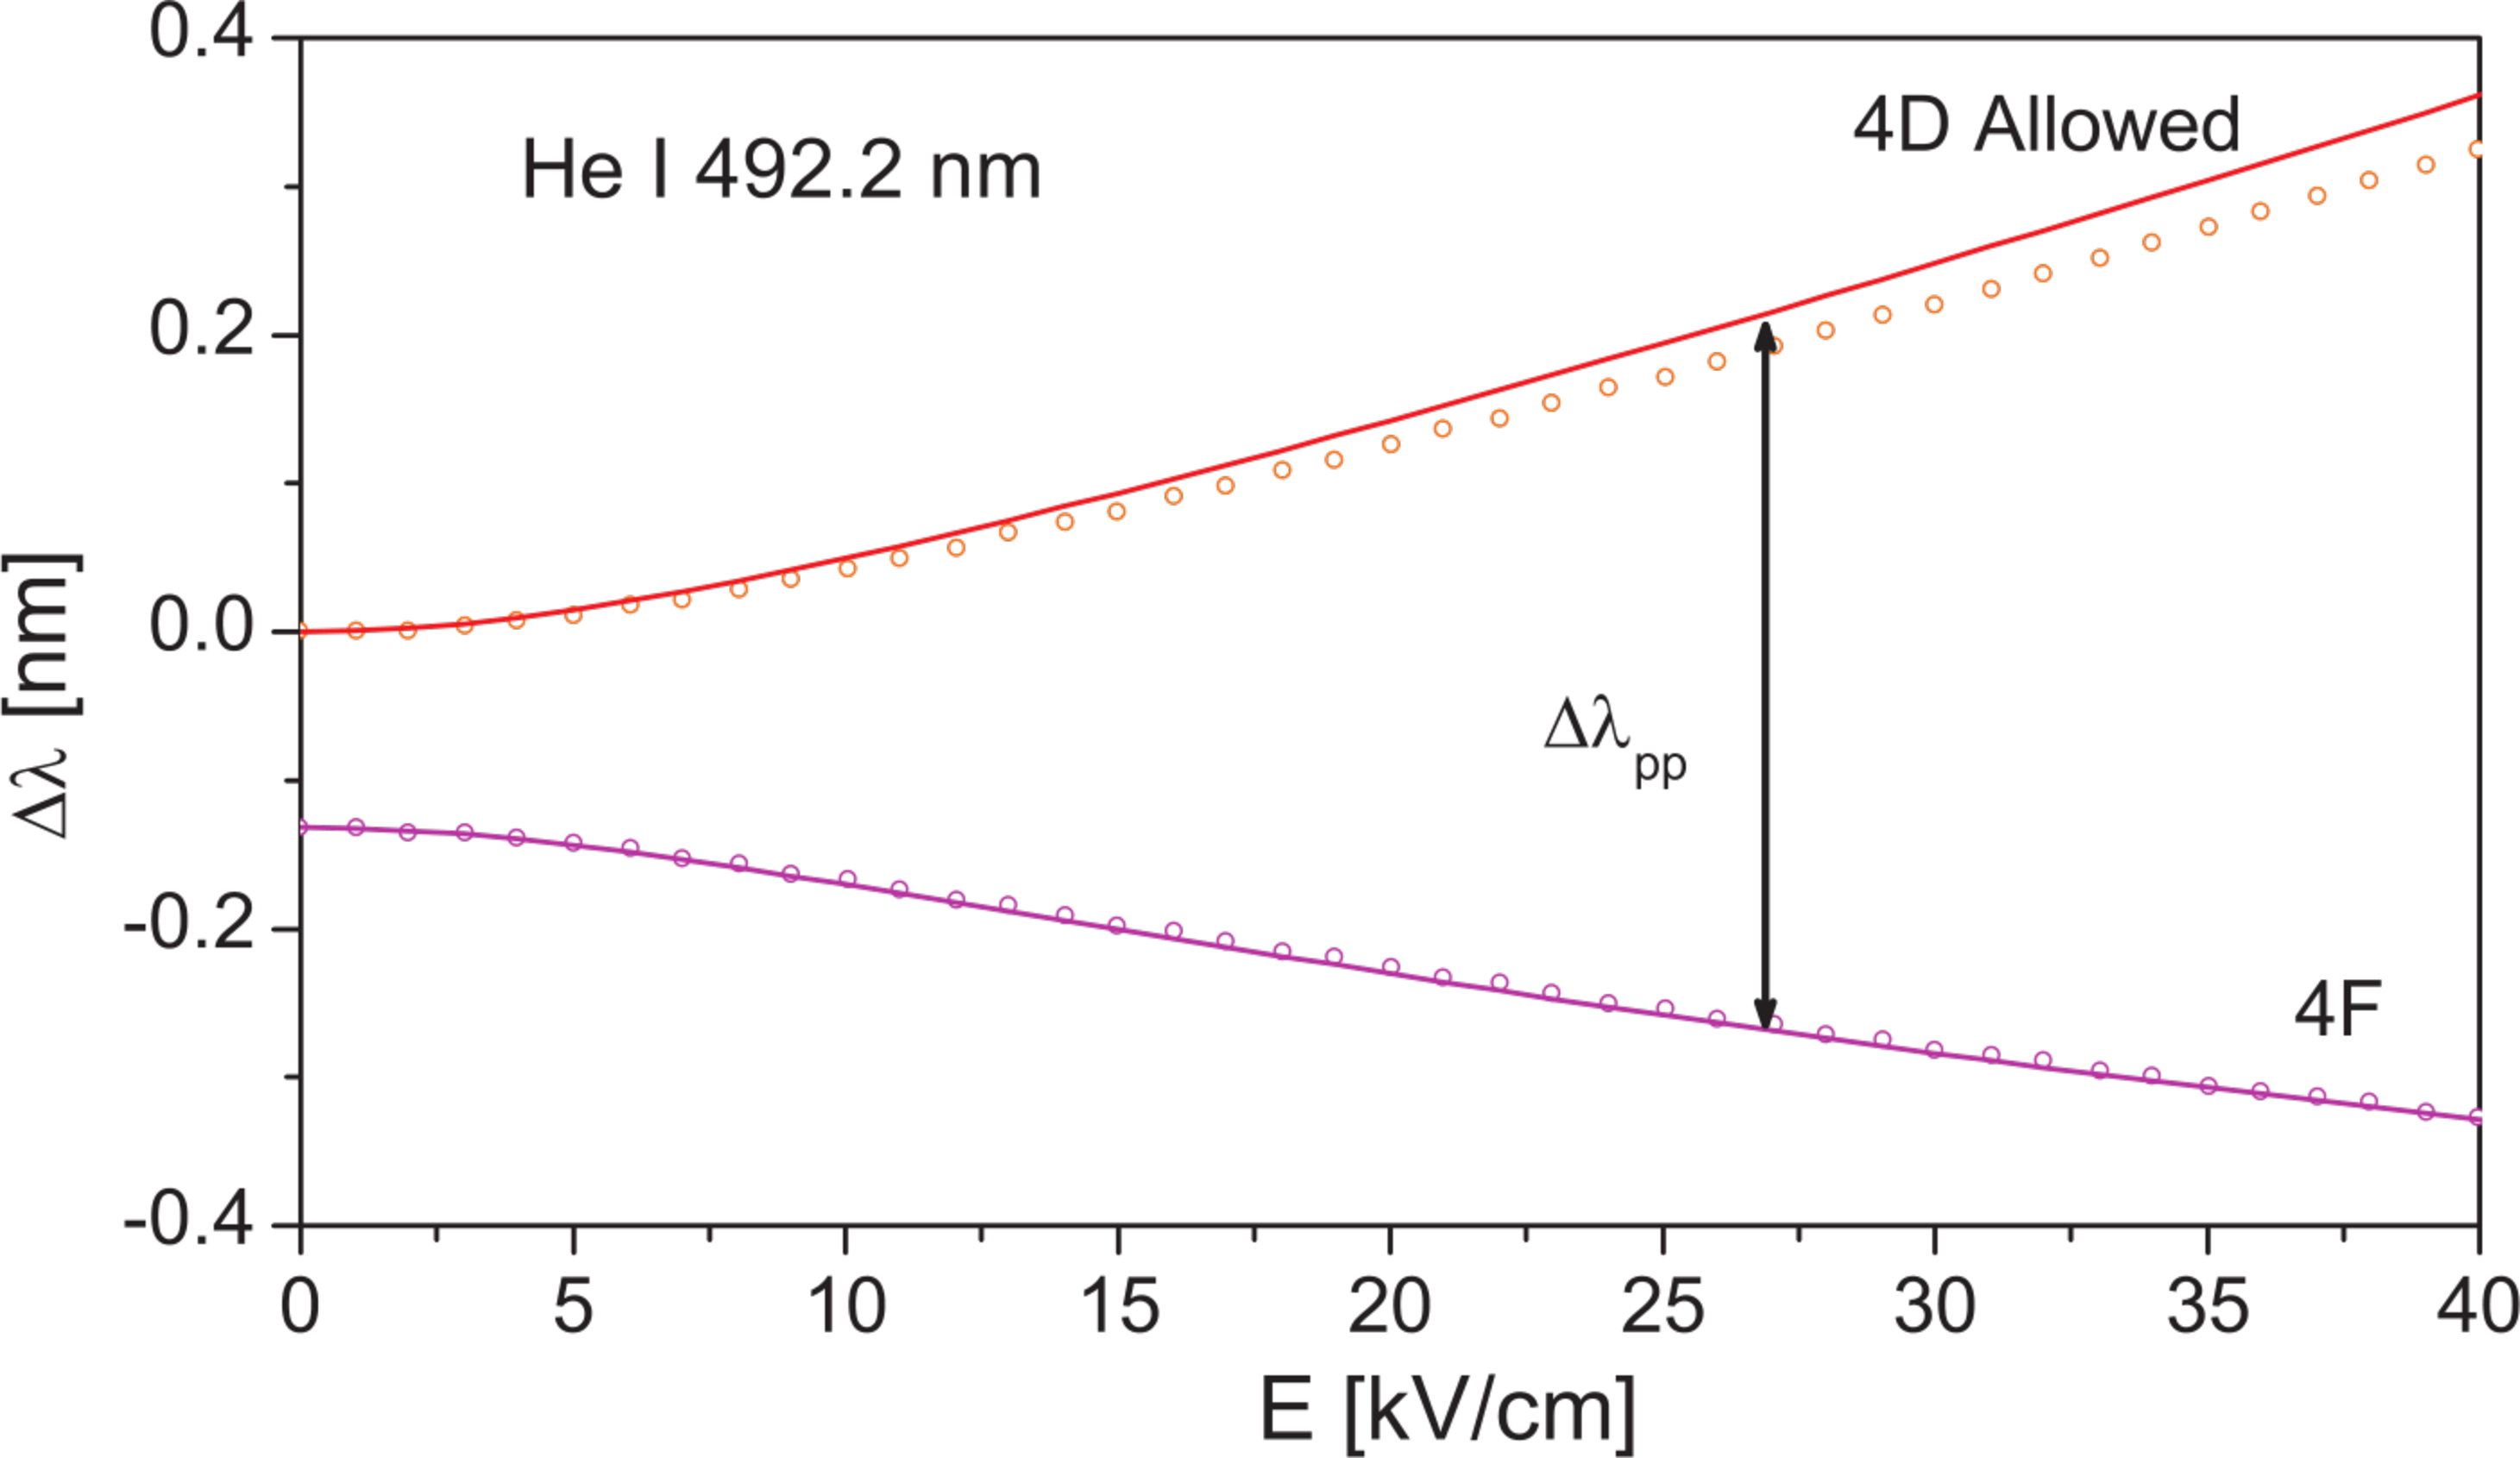
\includegraphics[width=0.5\textwidth]{figures/stark/starkshiftfielddependence.pdf}
					\caption{Calculated field dependences of $\Pi$-component shift. Wavelength shift is given with respect to the non-shifted allowed line. The difference in magnetic quantum number is coded with dots for $[1-1]$ or with solid lines for $[0-0]$ transitions. \cite{starkshiftmeas}}
					\label{img:fieldependence}
				\end{figure}
		
				\begin{figure}
					\centering
					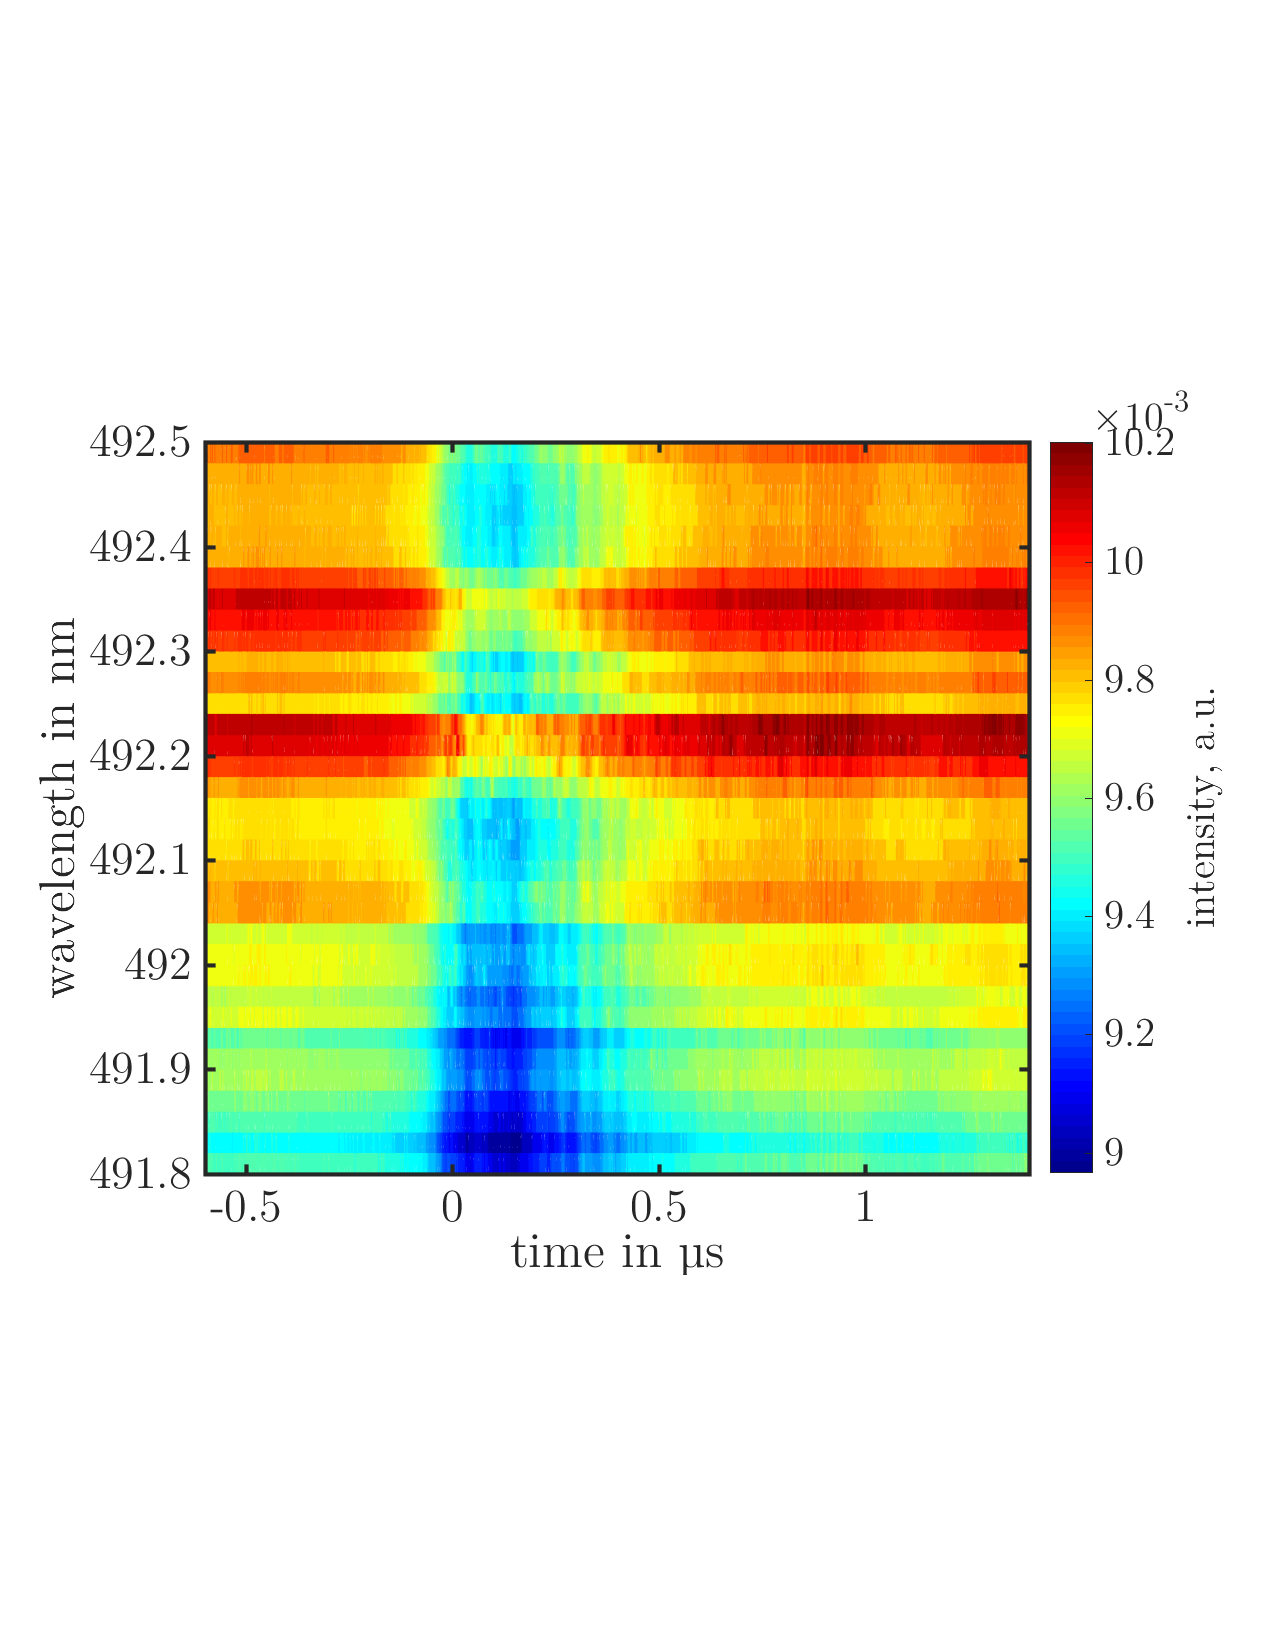
\includegraphics[width=0.5\textwidth]{figures/stark/stark_71inraw.pdf}
					\caption{Raw data from the temporally resolved stark spectroscopy at a vertical position of $\unit[7,1]{inch}$. The gathered information have not been processed any further, as only to be displayed here.}
					\label{img:rawdata}
				\end{figure}

				\begin{figure}
					\centering
					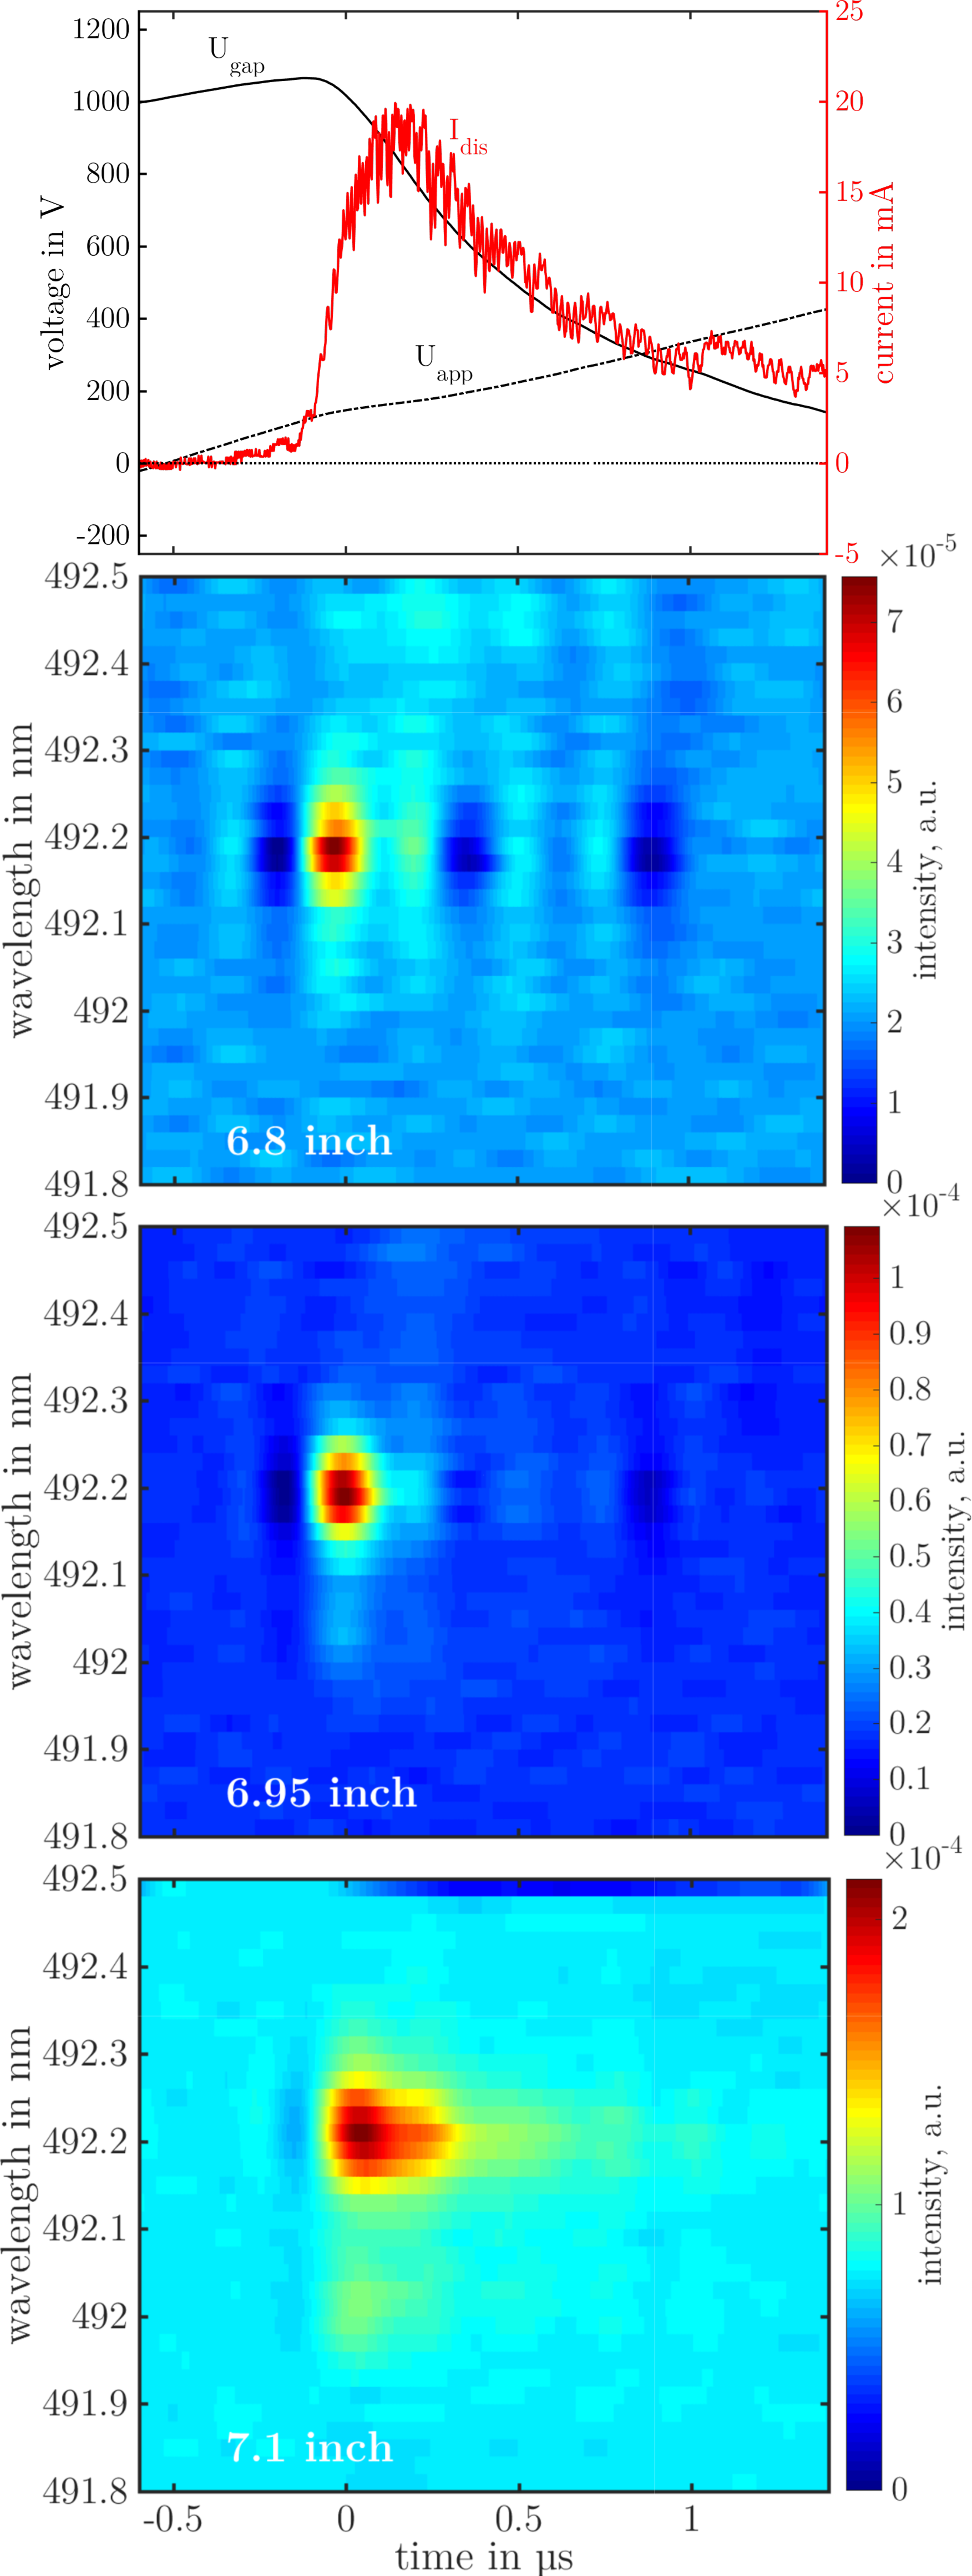
\includegraphics[width=0.5\textwidth]{figures/stark/combinations/starkallheightscombination.pdf}
					\caption{Comparison of the dicharge properties and spectral emission during stark spectroscopy at a vertical position of $\unit[7,1]{inch}$. }
					\label{img:stark71comparison}
				\end{figure}

				\begin{figure}
					\centering
					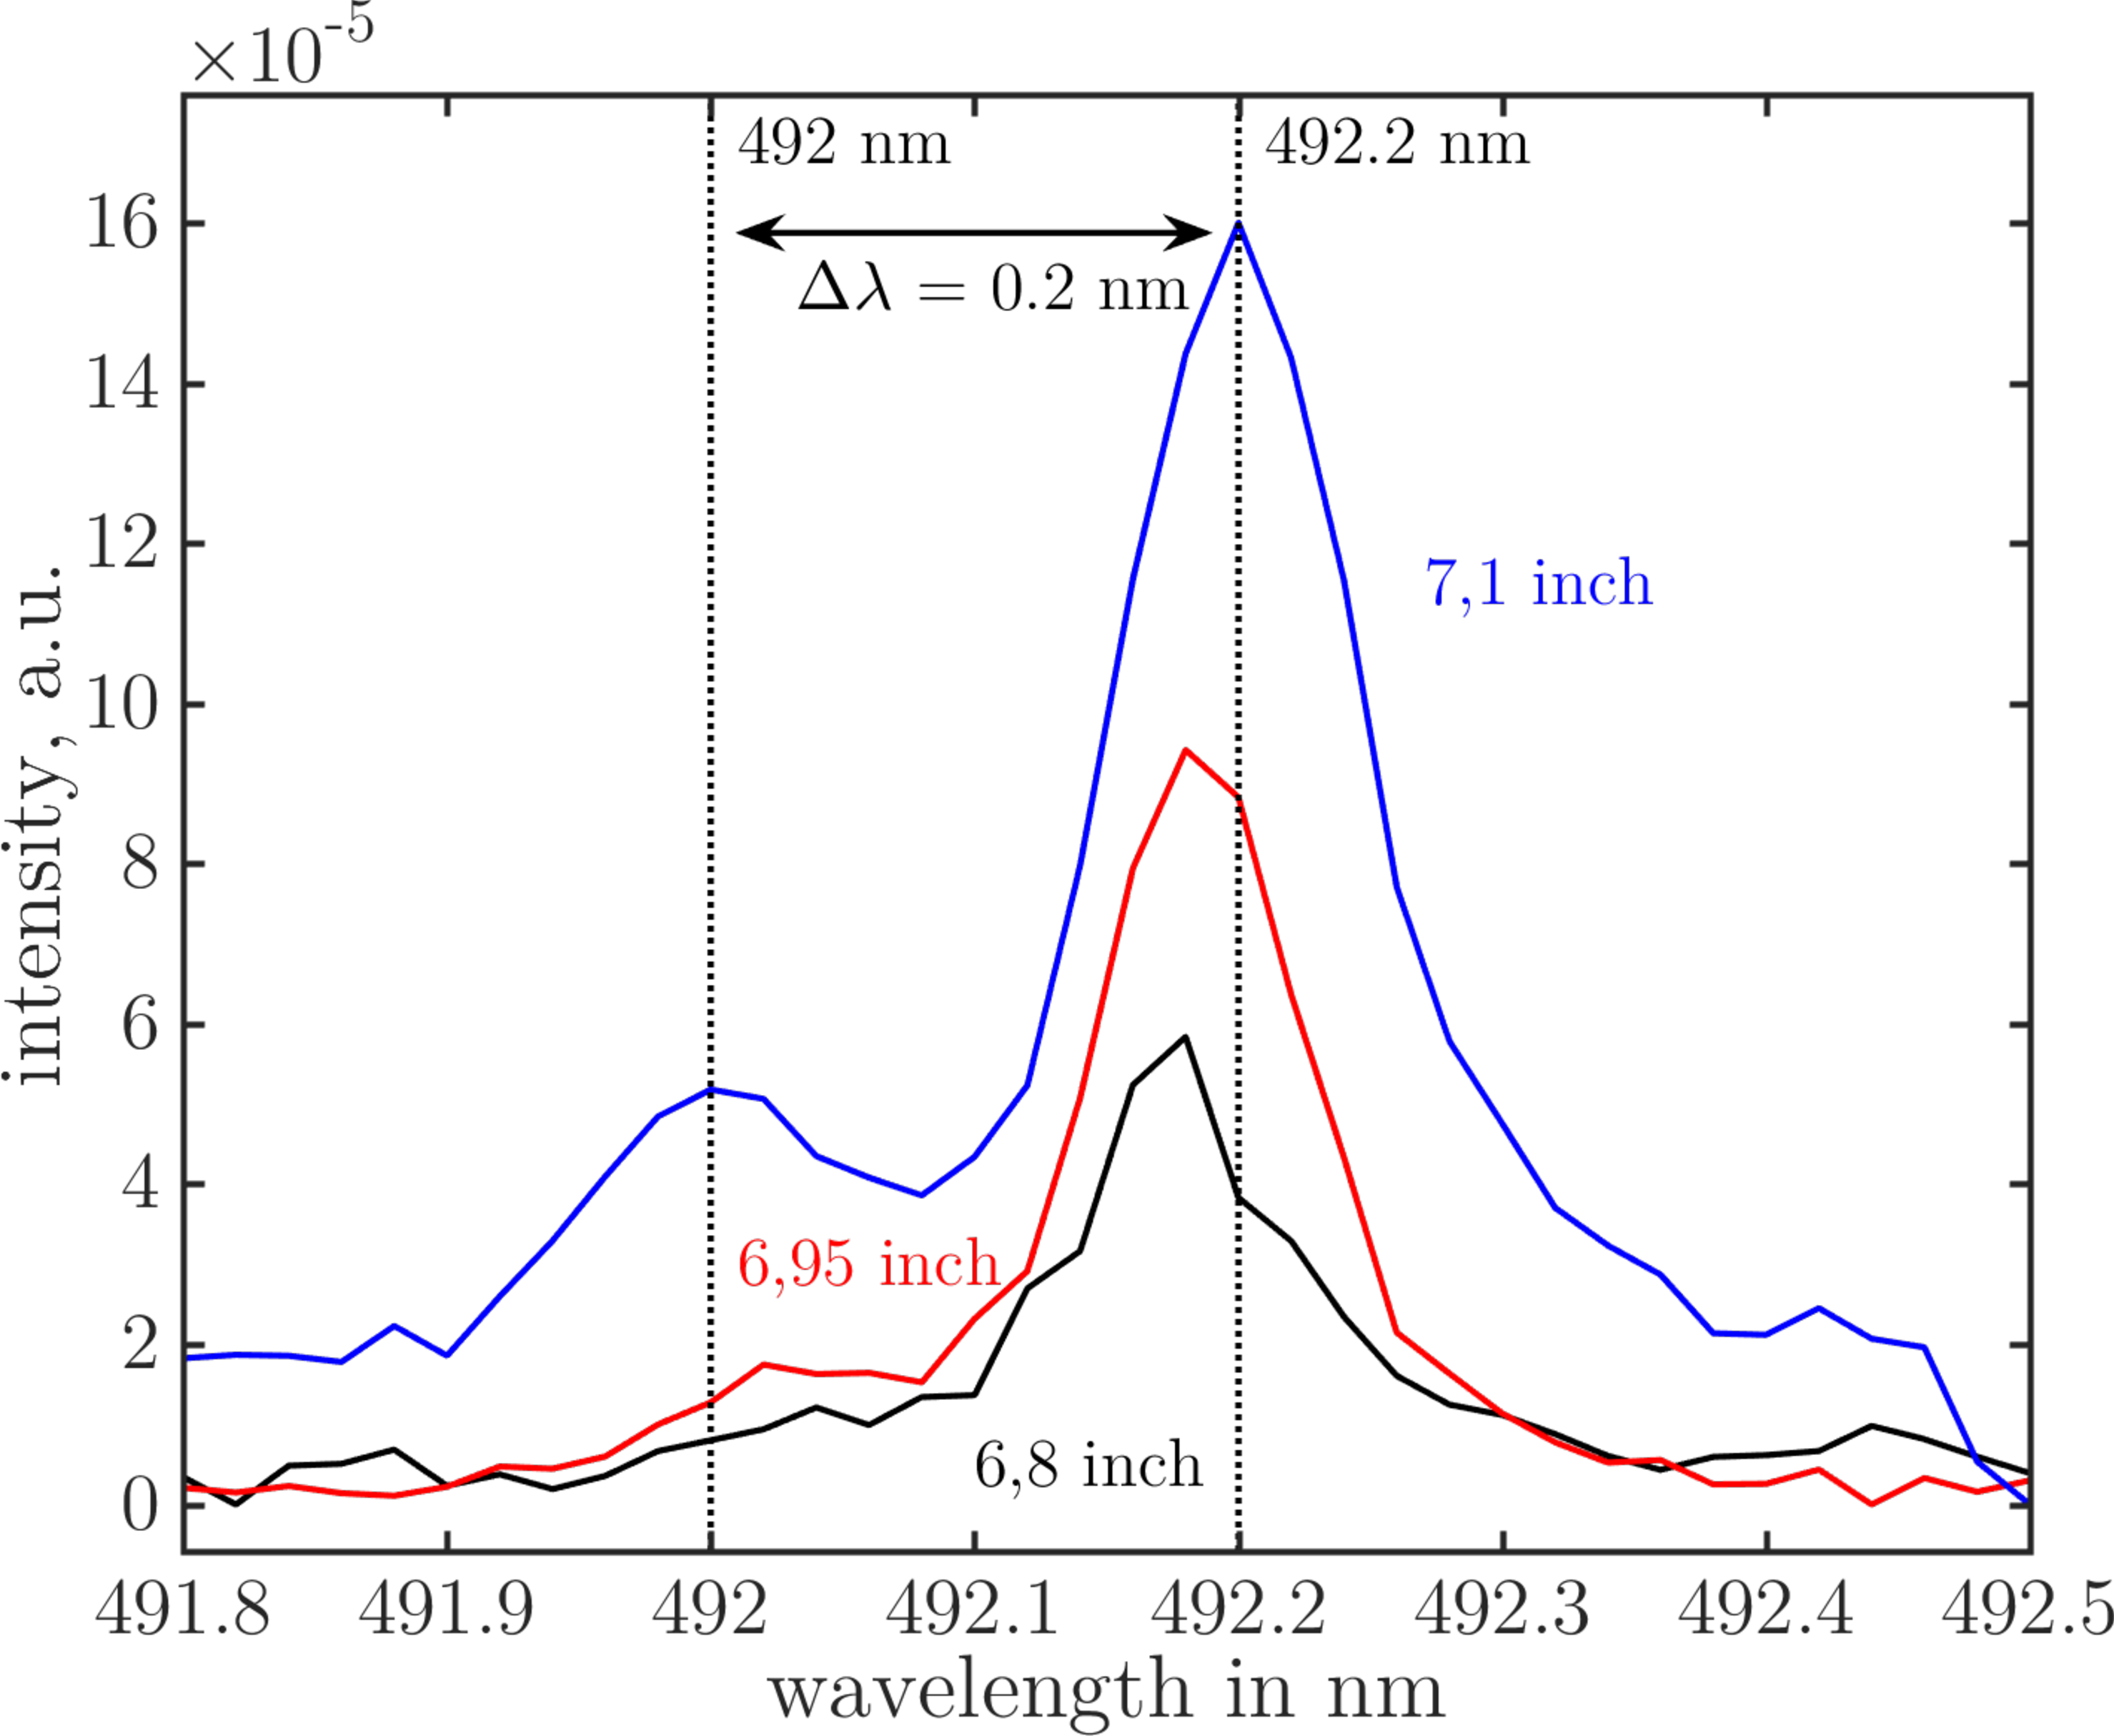
\includegraphics[width=0.5\textwidth]{figures/stark/combinations/stark_shiftallheights.pdf}
					\caption{Extracted emission profile around $\unit[492,2]{nm}$. This is at a relative time of $\unit[0,074]{\mu s}$ to the discharges ignition at $\unit[0]{\mu s}$.}
					\label{img:starkshift71}
				\end{figure}

	\section{Summary and outlook}
		
	\clearpage
		
	\section{Literature}

		\bibliography{report.bib}
		\bibliographystyle{plain}
		
	\section{Appendix}


\end{document}